\documentclass[11pt]{article}
\usepackage[margin=1in]{geometry}
\usepackage{graphicx}
\usepackage[utf8]{inputenc}
\usepackage[T1]{fontenc}
\usepackage{lmodern}
\usepackage{hyperref}
\usepackage{natbib}
\usepackage{xcolor}
\usepackage{booktabs}
\usepackage{longtable}
\usepackage{parskip}
\usepackage{enumitem}
\usepackage{caption}
\usepackage{amsmath}

\hypersetup{
    colorlinks=true,
    linkcolor=blue!60!black,
    citecolor=blue!60!black,
    urlcolor=blue!60!black
}

\title{\textbf{SSWD-EvoEpi: Modeling Sea Star Wasting Disease\\and Sunflower Star Recovery}\\[0.5em]\Large Progress Report}
\author{Willem Weertman \and Anton Star (AI Research Assistant)}
\date{March 2026}

\begin{document}

\maketitle

\section{Introduction}

Sea star wasting disease (SSWD) is one of the most devastating marine wildlife epidemics in recorded history. Beginning in 2013 along the Pacific coast of North America, the disease reduced populations of the sunflower sea star (\textit{Pycnopodia helianthoides}) by an estimated 90.6\% across its entire range, from Alaska to Baja California \citep{gravem2021}. In the southern portion of its range---California and Baja---the species was effectively eliminated. \textit{Pycnopodia} is now listed as Critically Endangered by the IUCN, a first for a sea star.

The cause of SSWD has been debated for over a decade. A major breakthrough came in 2025 when Prentice et al.\ published work in \textit{Nature Ecology \& Evolution} confirming the bacterium \textit{Vibrio pectenicida} as a strong candidate pathogen, satisfying Koch's postulates---the gold-standard criteria for establishing that a specific microbe causes a specific disease \citep{prentice2025}. This identification gives us, for the first time, a concrete biological agent to model.

The ultimate goal of this project is practical: \textit{Pycnopodia} captive breeding programs are underway, and wildlife managers need guidance on where, when, and how many stars to release to give reintroduced populations the best chance of survival. To answer those questions, we need a model that captures the essential biology---not just averages, but the variation between individuals, the differences between locations, and the evolutionary dynamics of both the host and the pathogen.

This is why we chose an \textbf{agent-based model} (ABM). Unlike traditional epidemiological models that track populations as single numbers (e.g., ``50,000 susceptible individuals''), an ABM simulates individual sea stars, each with its own genetic makeup, infection status, and location. This approach is more computationally expensive, but it lets us capture three things that matter enormously for SSWD:

\begin{enumerate}[leftmargin=2em]
    \item \textbf{Individual variation:} Not all stars are equally susceptible. Some carry alleles that confer partial resistance, and we need to track how those alleles spread through the population.
    \item \textbf{Spatial heterogeneity:} A site in the cold, enclosed waters of Prince William Sound, Alaska, experiences very different disease dynamics than an exposed headland in southern California. Our model must capture those differences.
    \item \textbf{Evolution:} Both the host (developing resistance) and the pathogen community (adapting virulence to local conditions) are evolving in real time. An ABM can simulate this naturally.
\end{enumerate}

This progress report describes the current state of the model---its biological foundations, its structure, what it captures well, and what challenges remain.

\section{Model Overview}

\begin{figure}[ht]
    \centering
    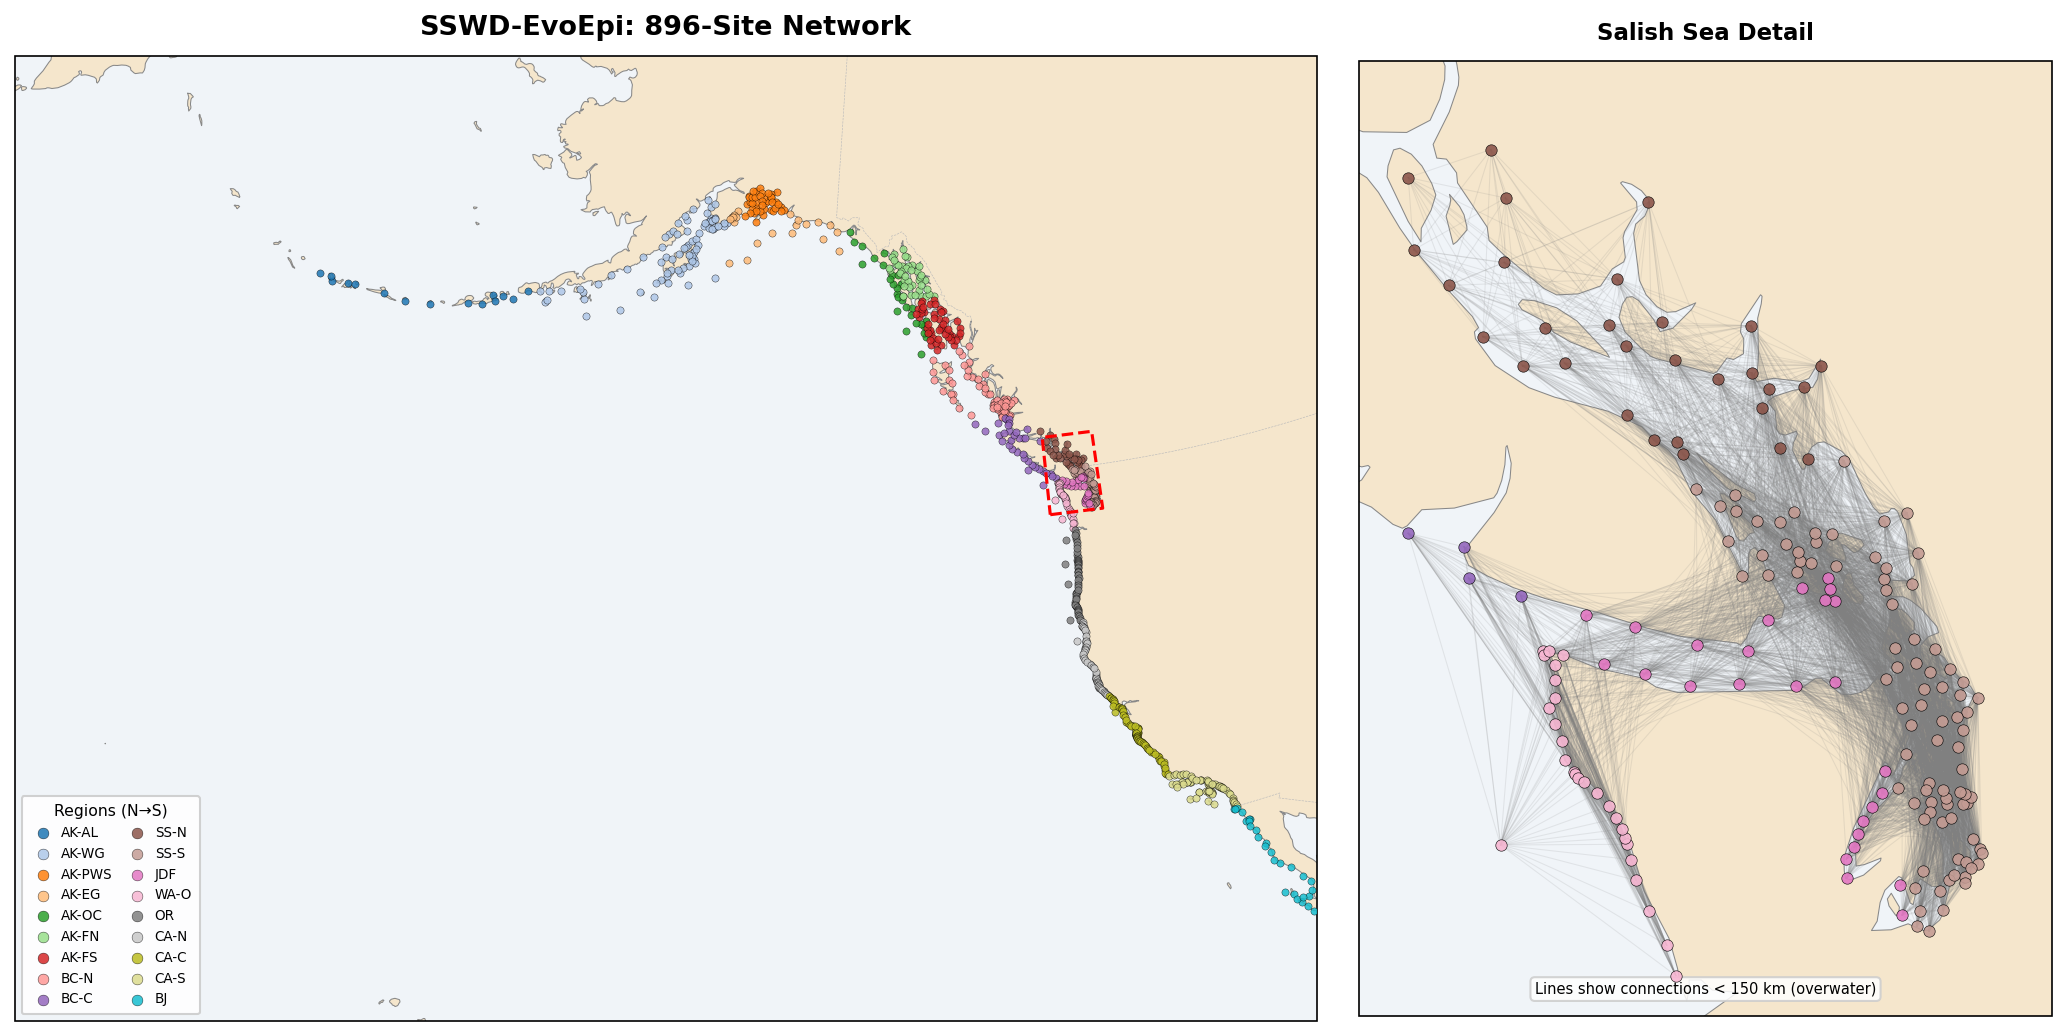
\includegraphics[width=0.85\textwidth]{figures/fig_network_map.png}
    \caption{The 896-site network spanning Alaska (Aleutians) to Baja California, colored by 18 geographic regions. The inset panel zooms into the Salish Sea, where connectivity lines (gray) show overwater connections between sites less than 150~km apart, illustrating the dense local network structure through which larvae and waterborne pathogen disperse.}
    \label{fig:network}
\end{figure}

The model simulates \textit{Pycnopodia} populations across \textbf{896 coastal sites} spanning the species' entire range, from the Aleutian Islands in western Alaska to Baja California, Mexico (Figure~\ref{fig:network}). These sites are grouped into 18 geographic regions that correspond to major oceanographic and biogeographic boundaries---for example, Prince William Sound, the Salish Sea, the Oregon coast, and the Channel Islands.

Each site can support up to \textbf{5,000 individual sea stars} (its ``carrying capacity''). At the start of the simulation, every site begins at full capacity, reflecting pre-disease conditions. Each individual star carries its own set of genes influencing disease resistance (described in Section 3b).

A critical design decision was to drive the model with \textbf{real sea surface temperature (SST) data} from the NOAA Optimum Interpolation SST dataset (OISST), which provides daily satellite-derived temperatures on a 0.25\textdegree\ grid from 2012 through 2024. We did not invent temperature scenarios---every site in the model experiences the actual temperatures that were measured at that location during each month of the simulation. This means that real climate events like El Ni\~no and La Ni\~na are automatically incorporated.

The simulation runs in \textbf{daily timesteps} over 13 years (2012--2025). Each day, the model steps through disease transmission, individual survival or death, and growth; reproduction and larval dispersal are resolved seasonally within the daily loop. The key biological insight underlying the entire model is that \textbf{temperature drives everything}: it determines when the pathogen becomes active, how fast disease spreads, and when stars reproduce.

\section{How Individuals and Sites Are Modeled}

\subsection{Individual Sea Stars}

Each of the up to 5,000 individuals at a site is modeled as a distinct entity with its own attributes. Every star has a \textbf{position} within the site (x, y coordinates in meters), a \textbf{heading} (direction of travel), \textbf{body size} (arm-tip diameter in mm, growing via von Bertalanffy dynamics), \textbf{age}, \textbf{sex}, and a \textbf{disease state} (susceptible, exposed, pre-symptomatic, symptomatic, or dead). Each individual also carries \textbf{51 genetic loci} (described in Section~\ref{sec:genetics}) that determine its resistance, tolerance, and recovery ability.

\begin{figure}[ht]
    \centering
    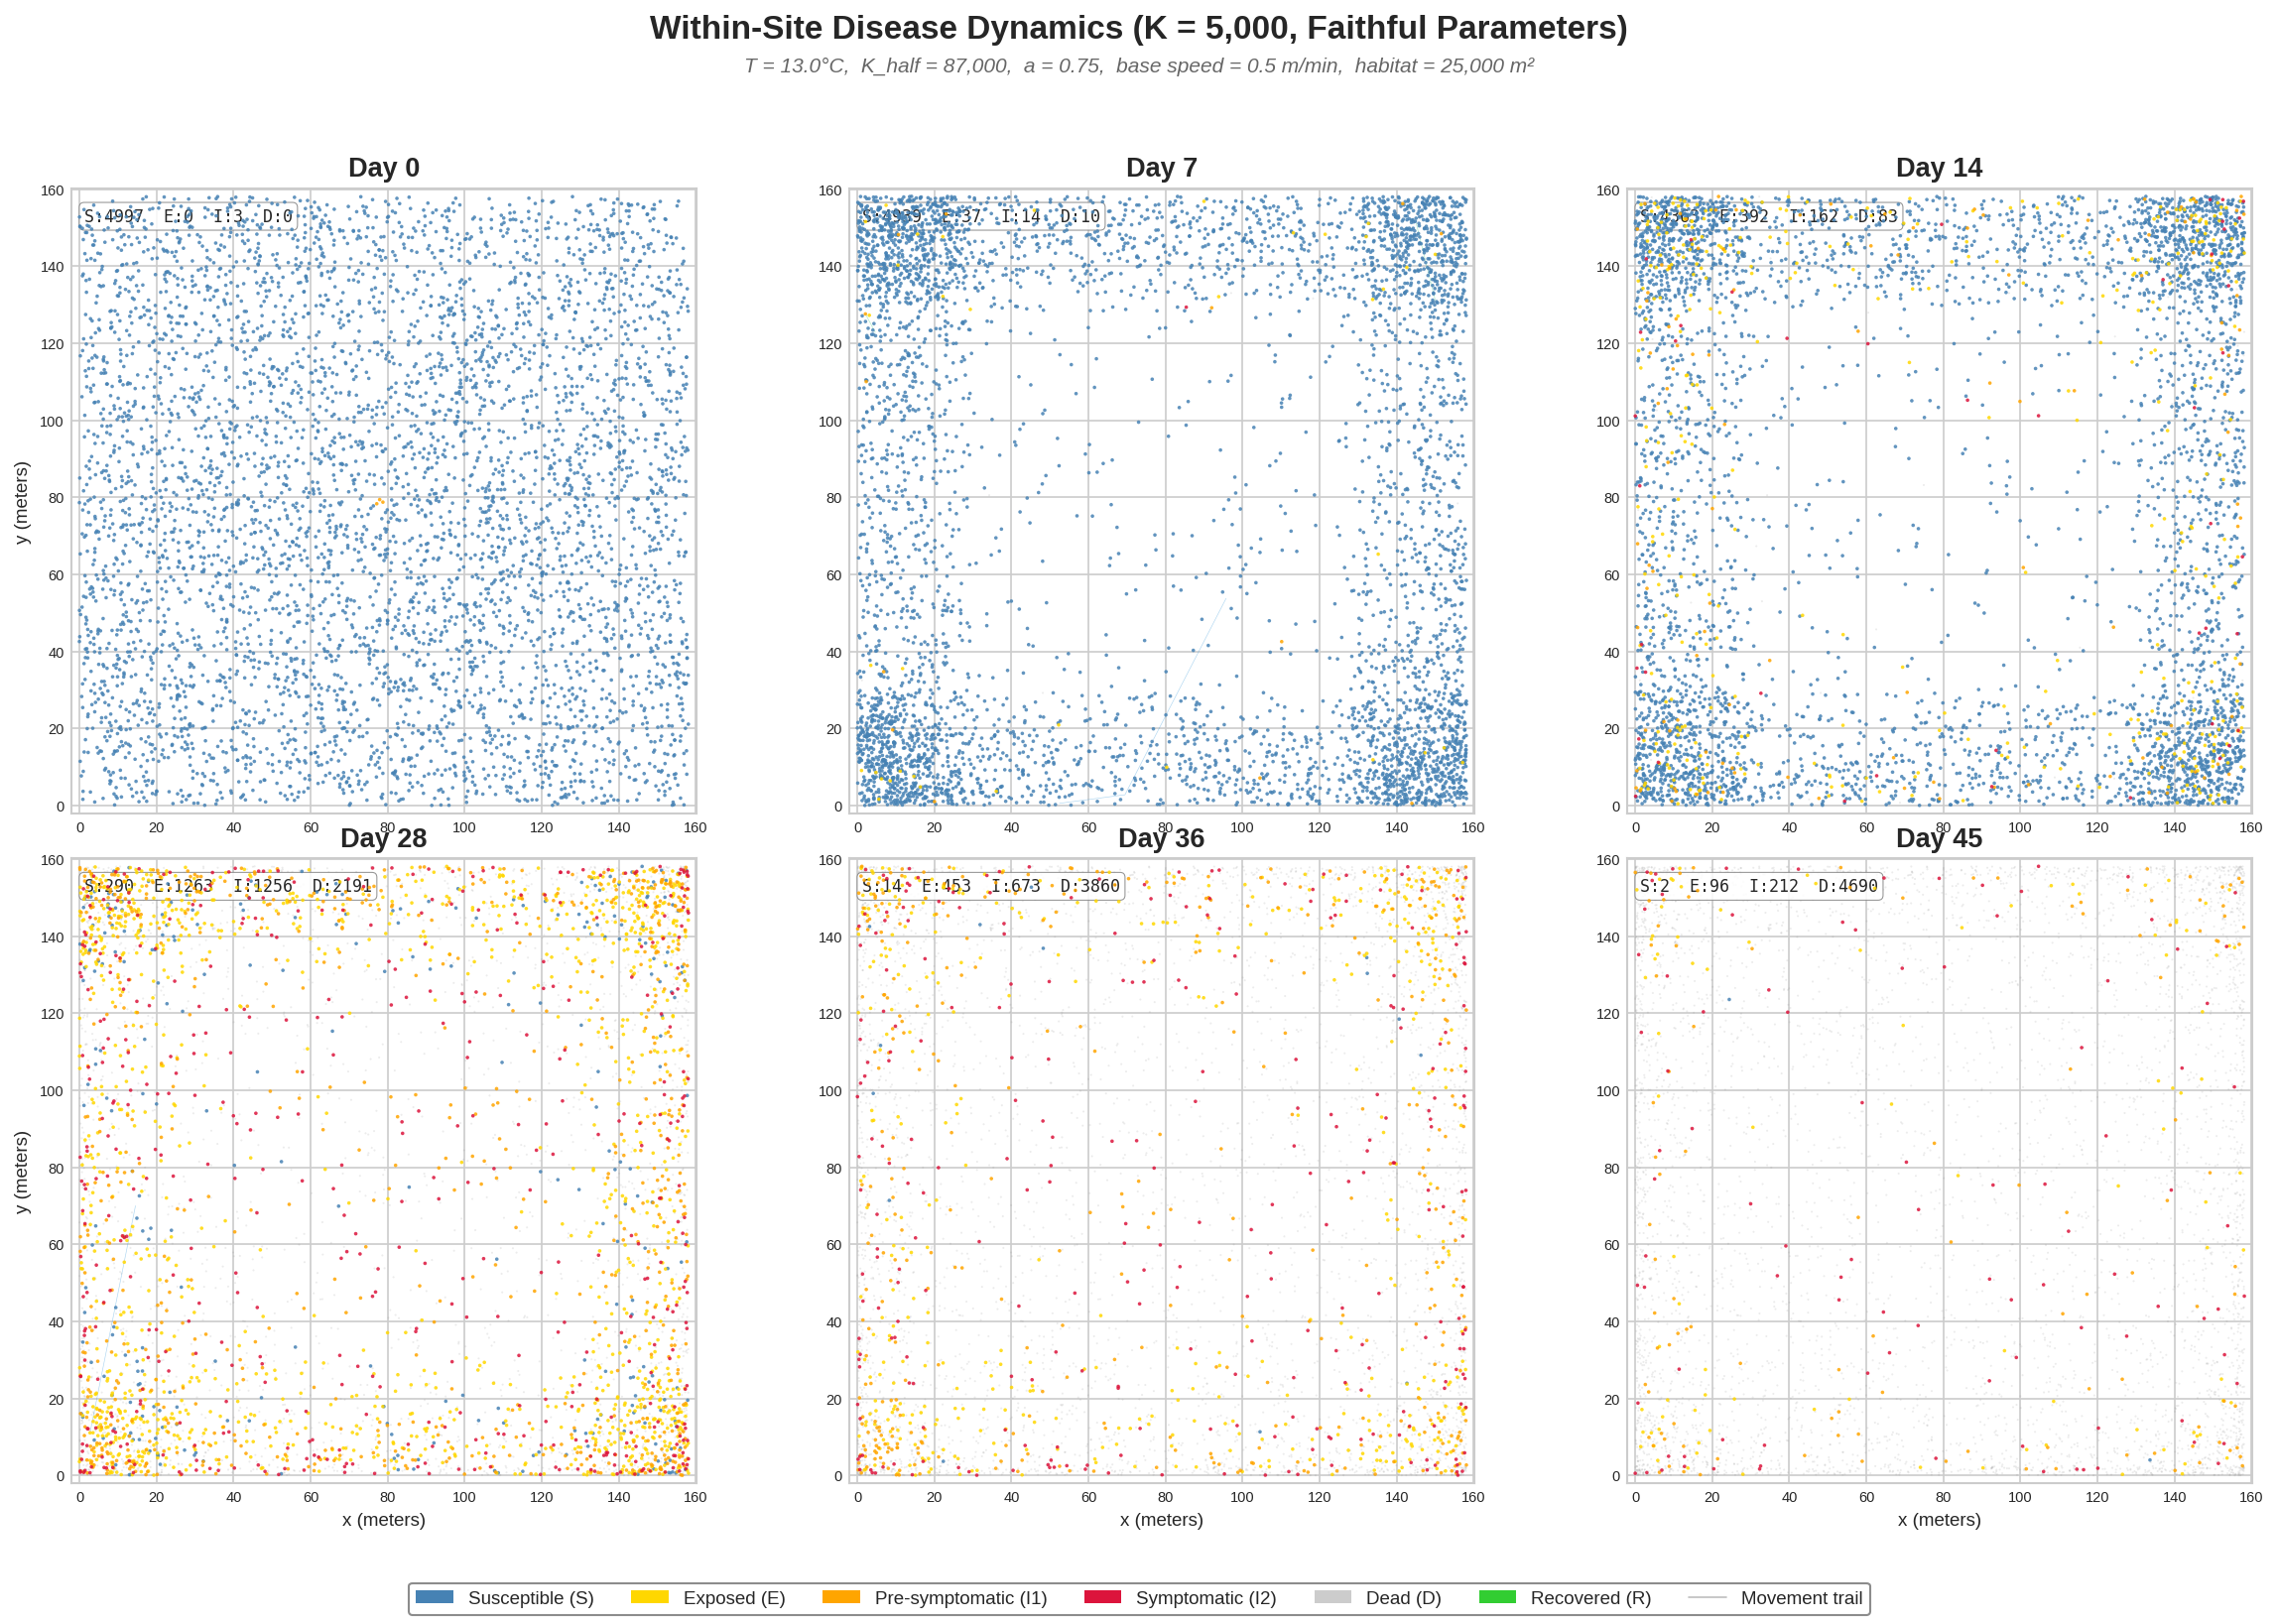
\includegraphics[width=0.95\textwidth]{figures/fig_within_site_disease.png}
    \caption{Simulated disease spreading through a single site using the model's actual transmission mechanics ($K = 5{,}000$ individuals, 158$\times$158~m habitat, $T = 13$\textdegree C). All parameters match the production model: correlated random walk movement (0.5~m/min base speed, 24 hourly substeps), grid-based spatial transmission (20~m cells with diffusion smoothing), dynamic environmental pathogen pool ($\alpha_{\text{env}} = 0.18$, $\delta_{\text{env}} = 0.05$), Hill-type force of infection ($K_{\text{half}} = 87{,}000$, $a = 0.75$), and Arrhenius-scaled disease progression. Disease begins with 3 pre-symptomatic individuals (Day~0). By Day~7, local spread is visible near the initial cluster. By Day~14, exposed (gold) and infected (orange/red) individuals are spreading across the site as the pathogen pool builds through positive feedback: more infected $\to$ more shedding $\to$ higher $P_k$ $\to$ more infections. Day~28 is peak infection (1{,}256 active infected). By Day~45, 93.8\% of the population is dead. Zero individuals recovered---consistent with the very low initial recovery ability ($\bar{c} = 0.02$). The rapidity of collapse at this density contrasts sharply with low-density populations, where the same parameters produce only $\sim$12\% mortality over 60 days, illustrating how density drives the positive feedback between host shedding and environmental pathogen accumulation.}
    \label{fig:within_site}
\end{figure}

\subsection{Movement: Correlated Random Walk}

Within each site, individuals move via a \textbf{correlated random walk} (CRW)---a standard model for animal movement in ecology. At each substep, a star's heading is perturbed by a random turn drawn from a normal distribution ($\sigma_{\text{turn}} = 0.6$ radians), and it advances at its current speed in the new direction. This produces realistic meandering paths with directional persistence: stars tend to keep going roughly the same way, with gradual course changes.

\textbf{Movement speed} is based on field observations of \textit{Pycnopodia} locomotion \citep{hodin2021}: a base speed of 0.5~m/min (approximately 30~m/hr), which is modified by disease state:
\begin{itemize}[leftmargin=2em]
    \item Healthy and exposed stars move at full speed
    \item Pre-symptomatic (I$_1$) stars slow to 50\% of normal
    \item Symptomatic (I$_2$) stars slow to 10\% of normal---they are visibly wasting
    \item Dead stars do not move
\end{itemize}

Movement is resolved in \textbf{24 hourly substeps per day}, meaning each star takes 24 movement steps in a simulated day. The habitat at each site is represented as a square arena (side length $\approx 158$~m for a 25,000~m$^2$ habitat), with elastic boundary reflection---stars that would walk off the edge bounce back.

\subsection{Spatial Disease Transmission Within Sites}

Movement matters because disease transmission is \textbf{spatially explicit within each site}. Rather than assuming every susceptible individual encounters the same pathogen concentration (the ``well-mixed'' assumption), the model tracks where infected individuals are located on a 20~m grid. Susceptible stars that happen to be near clusters of infected individuals experience higher local pathogen exposure, while those farther away experience lower exposure. This creates realistic spatial clustering of disease outbreaks within a site---an infected star sheds pathogen that first affects its immediate neighbors, producing a local wave of infections.

\subsection{Pre-Spawning Aggregation}

Before the spawning season, stars exhibit \textbf{gravity-like attraction} toward nearby conspecifics, mimicking the aggregation behavior observed in broadcast spawners. For 14 days before (and 14 days after) spawning readiness, an individual's movement heading is gently biased toward the nearest conspecific within a 100~m detection range. This pre-spawning aggregation increases local density, improving fertilization success---but it also brings individuals into closer proximity, which can accelerate disease transmission.

\subsection{Density-Dependent Fertilization and Allee Effects}

Because sunflower stars are broadcast spawners---releasing eggs and sperm into the water---\textbf{fertilization success depends on local adult density}. In a large, healthy population, sperm encounters eggs readily. But as population density drops (for instance, after a disease crash), the probability that a given egg encounters sperm decreases. This is the classic \textbf{Allee effect} in broadcast spawners.

We implement this using the Lundquist \& Botsford (2004) fertilization kinetics model:

\begin{center}
$F(\rho) = 1 - e^{-\gamma \times \rho_{\text{eff}}}$
\end{center}

\noindent where $\rho_{\text{eff}}$ is the effective local male density (individuals per m$^2$) and $\gamma = 4.5$~m$^2$ is the sperm contact parameter. At high density, nearly all eggs are fertilized ($F \to 1$). At low density, fertilization collapses exponentially.

Two features mitigate the Allee effect. First, the \textbf{pre-spawning aggregation behavior} described above concentrates individuals into clumps, raising the effective local density above the site-wide average. When at least 20 adults aggregate, the effective density within clumps can reach 0.5~ind/m$^2$---dramatically improving fertilization even at low site-wide densities. Second, a \textbf{settlement cue modifier} reduces larval settlement success at sites with very few adults. Settlement follows a Michaelis--Menten curve from a baseline of 20\% (bare substrate, coralline algae cues only) to 100\% (full adult population providing chemical cues). This means that functionally extinct sites are harder for larvae to recolonize, creating a second Allee threshold at the settlement stage.

Together, these mechanisms create a \textbf{double Allee effect}: populations must be large enough both for adults to fertilize each other's gametes \textit{and} for the site to attract and retain settling larvae. A site that loses too many adults can enter an extinction vortex---too few spawners to fertilize eggs, too few adults to cue larval settlement, leading to further decline even after disease pressure abates. This is directly relevant to reintroduction planning: releasing individuals into a site with no surviving adults may require larger release cohorts to overcome these Allee thresholds.

\subsection{Site-Level Structure}

Each of the 896 sites is a self-contained population unit with its own:
\begin{itemize}[leftmargin=2em]
    \item \textbf{Carrying capacity} ($K = 5{,}000$ in current calibration, uniform across sites)
    \item \textbf{Daily sea surface temperature} (from real NOAA OISST satellite data)
    \item \textbf{Environmental pathogen pool} (dynamic, accumulating from local shedding and decaying daily)
    \item \textbf{Flushing rate} ($\varphi$), computed from the site's geographic enclosedness---enclosed waterways flush pathogen slowly; exposed coastline flushes quickly
    \item \textbf{Larval self-recruitment fraction} ($\alpha_{\text{self}}$), interpolated continuously from the enclosedness metric between 2\% (open coast) and 70\% (deep fjord)
    \item \textbf{Evolving pathogen traits}: each site's bacterial community has its own thermal activation threshold and virulence, which drift over time in response to local conditions
\end{itemize}

Sites are connected to each other through two dispersal kernels: a \textbf{larval dispersal kernel} ($D_L = 400$~km, exponential decay) that moves larvae between sites during reproduction, and a \textbf{pathogen dispersal kernel} ($D_P = 15$~km, exponential decay) through which waterborne pathogen spreads between neighboring sites daily.

\section{Biology in the Model}

\subsection{Reproduction and Larval Dispersal}

Sunflower stars are broadcast spawners---they release eggs and sperm into the water column, where fertilization occurs externally. In the model, spawning timing is based directly on your published work \citep{hodin2021}. The spawning season runs from November through mid-July, with peak activity between November and March. Spawning timing shifts with latitude according to the relationship:

\begin{center}
\textit{Peak spawning day} = day 50 + 3 $\times$ (latitude $-$ 48.5\textdegree)
\end{center}

In plain terms: stars in Alaska spawn later in the season than stars in California. A population at 55\textdegree N (southern Alaska) would peak around day 70 (mid-March), while a population at 35\textdegree N (southern California) would peak around day 10 (mid-January). This matches field observations of latitudinal variation in reproductive timing.

After spawning, \textbf{larvae disperse} between connected sites. Rather than modeling individual larval trajectories through ocean currents (which would require a full hydrodynamic model), we use a simplified connectivity scheme based on distance between sites and coastal geometry. Nearby sites exchange more larvae than distant ones, and the connectivity decreases with distance according to an exponential decay function ($e^{-d/D_L}$, where $D_L = 400$ km is the characteristic dispersal scale).

One of the more novel features of the model is the \textbf{``enclosedness'' metric}. We algorithmically computed how geographically enclosed each site is based on the surrounding coastline geometry. A site deep inside Puget Sound or a Norwegian-style fjord in British Columbia scores high on enclosedness; an exposed outer-coast site scores low.

Enclosedness affects the model in two important ways that create an inherent trade-off:
\begin{itemize}[leftmargin=2em]
    \item \textbf{More larval retention:} Enclosed waterways trap larvae, meaning local reproduction contributes more to local recruitment. This is good for population recovery.
    \item \textbf{More pathogen retention:} The same physical enclosure that retains larvae also traps waterborne pathogen. This is bad for disease escape.
\end{itemize}

Finally, \textbf{settlement survival} is set at 0.1\%---meaning only 1 in 1,000 larvae that settle at a site survive to become juveniles. This is consistent with the extremely high larval mortality rates observed across marine invertebrates, where producing millions of larvae to yield a handful of recruits is the norm.

\subsection{Sweepstakes Reproductive Success}

The reproductive system in the model is built around the concept of \textbf{sweepstakes reproductive success} (SRS), inspired by the Hedgecock hypothesis \citep{hedgecock2011}. In many marine broadcast spawners, reproductive success is not evenly distributed among adults. Instead, a small fraction of individuals ``win the lottery'' in any given spawning event---their gametes happen to meet at the right time, in the right place, under favorable conditions---while most adults contribute nothing to the next generation.

We implement this explicitly using a \textbf{Pareto-weighted random lottery}. When spawning occurs at a site, each reproductively active female and male receives a random weight drawn from a Pareto distribution (shape parameter $\alpha = 1.35$). This heavy-tailed distribution means that a few individuals receive very large weights while most receive small ones. Females are additionally weighted by body-size-dependent fecundity---larger females produce more eggs.

Parent pairs are then sampled with replacement from these weighted distributions to produce offspring. The result is that in any given spawning event, a handful of parents may contribute disproportionately to the next cohort, while many adults contribute no surviving offspring at all.

This has important evolutionary consequences:
\begin{itemize}[leftmargin=2em]
    \item \textbf{Genetic drift is amplified:} The effective population size ($N_e$) is much smaller than the census population, meaning allele frequencies can shift rapidly by chance---not just by selection.
    \item \textbf{Rapid trait change is possible:} If, by chance, a disease-resistant individual ``wins'' the reproductive lottery, its alleles can sweep through the local population in just a few generations, even without strong directional selection.
    \item \textbf{Variance in outcomes:} Different random seeds can produce quite different evolutionary trajectories at the same site, mirroring the real stochasticity observed in marine population genetics.
\end{itemize}

This mechanism is particularly important for understanding post-disease recovery. In a depleted population where only a few dozen adults survive, the sweepstakes lottery means that recovery genetics depend heavily on \textit{which} individuals happen to reproduce successfully---not just how many survive.

\subsection{Host Genetics and Evolution}
\label{sec:genetics}

\begin{figure}[ht]
    \centering
    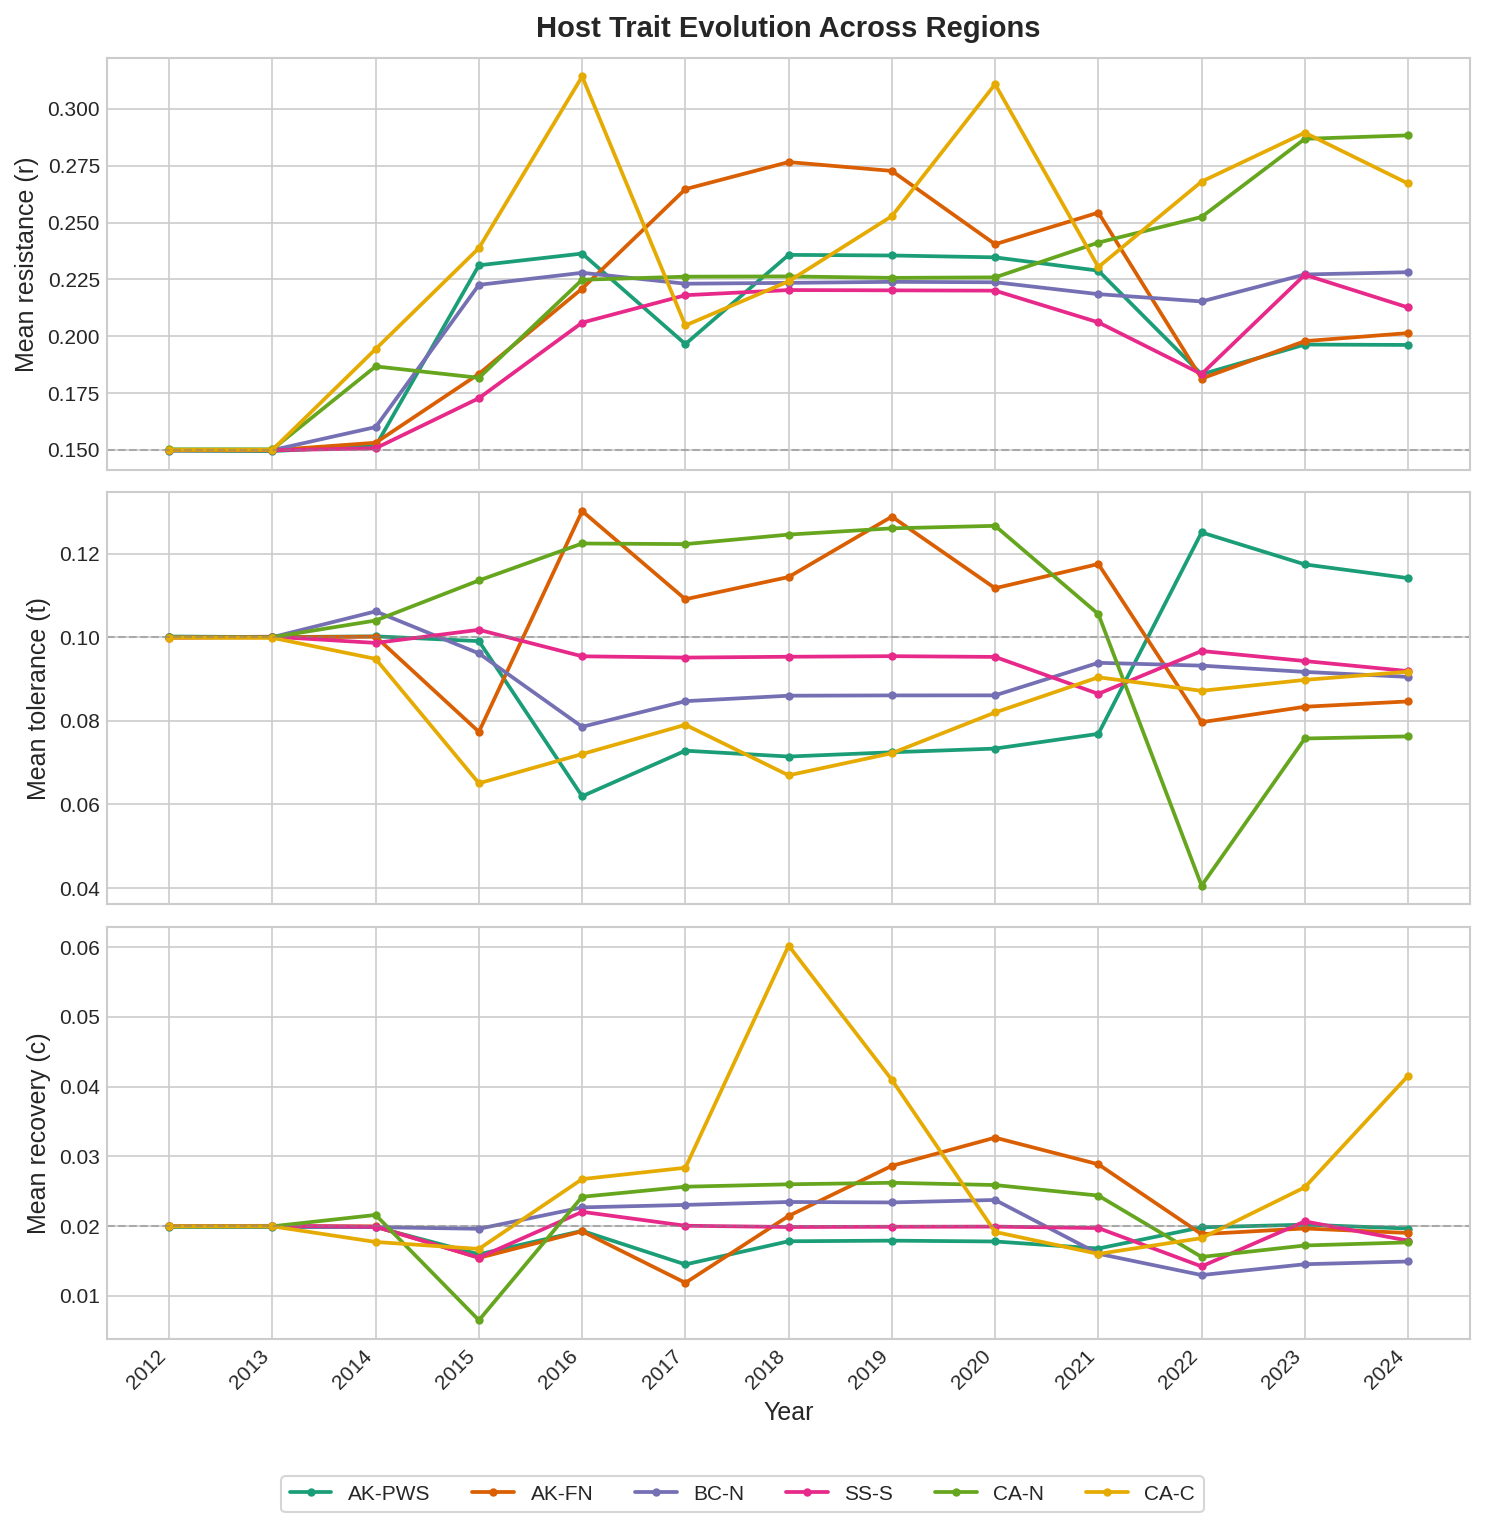
\includegraphics[width=0.90\textwidth]{figures/fig_all_traits_evolution.png}
    \caption{Evolution of all three host defense traits across six representative regions over 13 years. \textbf{Top:} Resistance ($r$) increases under selection, with southern regions evolving fastest. \textbf{Middle:} Tolerance ($t$) shows complex, region-dependent trajectories---some populations increase tolerance while others decrease it, reflecting different selective regimes. \textbf{Bottom:} Recovery ($c$) remains near its initial value in most regions but increases substantially in some southern populations under intense selection.}
    \label{fig:traits}
\end{figure}

\begin{figure}[ht]
    \centering
    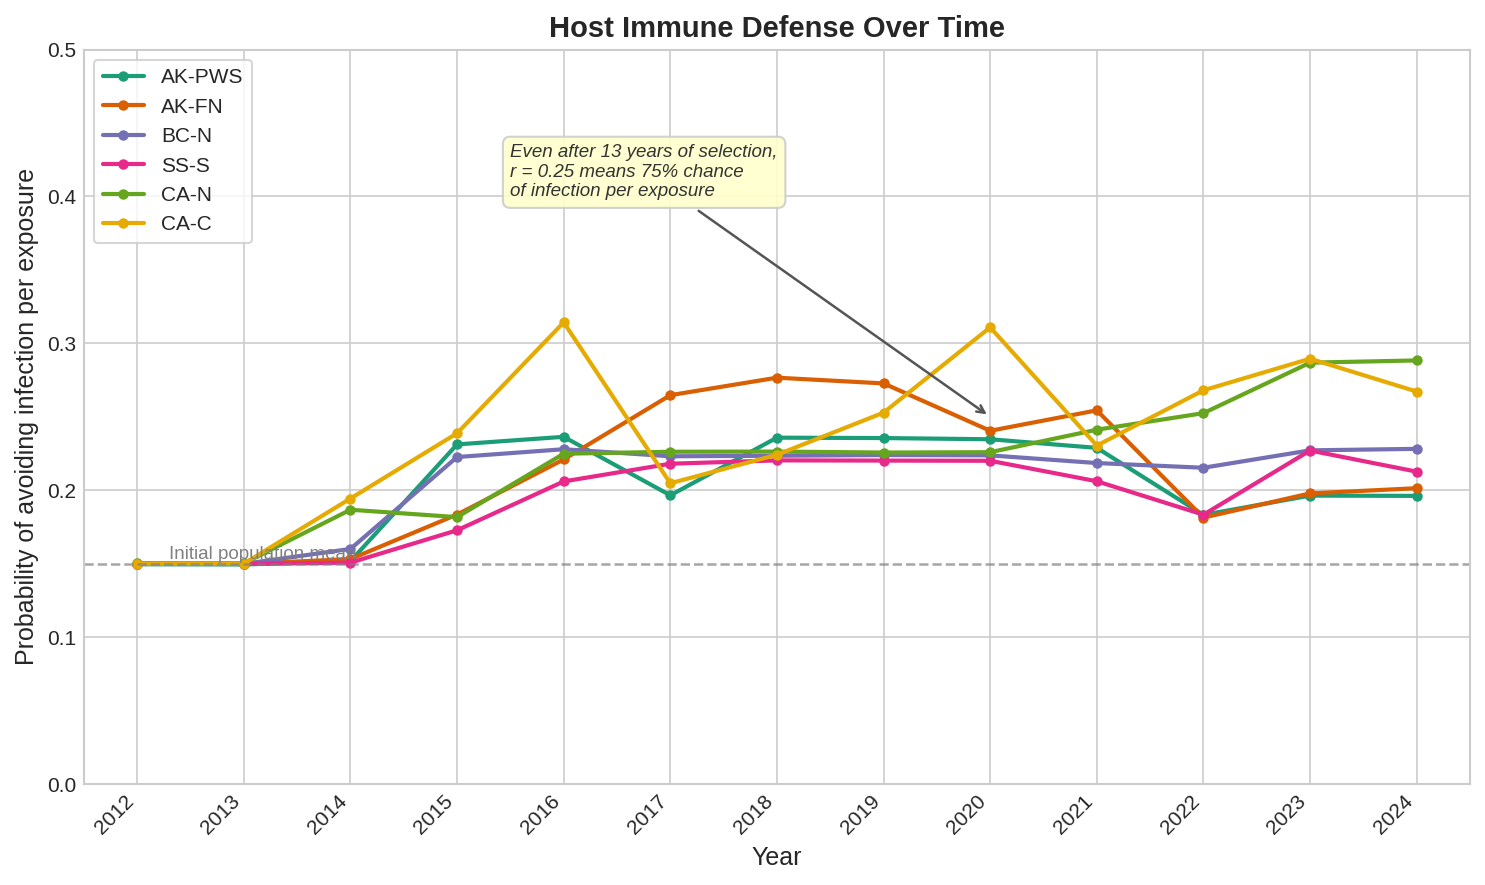
\includegraphics[width=0.85\textwidth]{figures/fig_survival_probability.png}
    \caption{Mean resistance trait ($r$) by region over time. Higher $r$ reduces the force of infection: a star with $r = 0.25$ experiences a 25\% reduction in its infection hazard rate compared to a fully susceptible individual. Despite 13 years of selection, even the most resistant regional populations only reach $r \approx 0.25$--$0.29$. Evolution is occurring but remains far too slow to outpace the epidemic.}
    \label{fig:survival}
\end{figure}

Each individual sea star in the model carries \textbf{51 genetic loci} (specific positions in the genome) that influence its ability to deal with disease. This genetic architecture is inspired by genome-wide association studies (GWAS) by Schiebelhut et al., which identified multiple genomic regions associated with SSWD survival in the ochre star \textit{Pisaster ochraceus}---a related asteroid species for which population genomic data is available. No equivalent GWAS data yet exists for \textit{Pycnopodia}, so we borrow this genetic architecture as a biologically grounded starting point.

The 51 loci are divided equally among three heritable defense traits:

\begin{enumerate}[leftmargin=2em]
    \item \textbf{Resistance ($r$):} Scales how susceptible an individual is to infection. In the model, each star's infection hazard rate is multiplied by $(1 - r)$, so a star with $r = 0.30$ faces a 30\% reduction in its instantaneous risk of infection compared to a fully susceptible individual. Think of it as an \textit{armor rating}---higher resistance means a substantially lower chance of becoming infected in any encounter with the pathogen. Each of the 17 resistance loci contributes additively (with exponentially distributed effect sizes, so a few loci have large effects and many have small ones).

    \item \textbf{Tolerance ($t$):} The ability to survive while infected. Tolerance reduces the rate at which symptomatic (I$_2$) individuals progress to death, effectively extending survival time during late-stage infection. A tolerant star lives longer with the disease, buying time for potential recovery. Think of it as \textit{toughness}---the star can take a hit and keep going.

    \item \textbf{Recovery ($c$):} Scales the daily probability of clearing the pathogen. The effective daily clearance rate is $\rho_{\text{rec}} \times c$, where $\rho_{\text{rec}} = 0.05$ is the base recovery rate. Think of it as a \textit{healing factor}---a star with high recovery can fight off an active infection and return to susceptible status (echinoderms lack adaptive immunity, so recovered individuals can be reinfected).
\end{enumerate}

At the start of the simulation, the population begins with low defense values: $r = 0.15$ (a 15\% reduction in infection hazard---still highly susceptible), $t = 0.10$, and $c = 0.02$ (giving an effective daily clearance rate of $0.05 \times 0.02 = 0.001$, or 0.1\% per day---recovery is extremely rare). These low starting values reflect the fact that \textit{Pycnopodia} populations were largely naive to this pathogen before the 2013 outbreak.

\textbf{Natural selection} operates straightforwardly: stars that survive disease are more likely to have favorable alleles at resistance, tolerance, and recovery loci. When these survivors reproduce, they pass those alleles to their offspring. Over generations, the population evolves higher average defense values.

Figure~\ref{fig:traits} shows how all three defense traits evolve across regions, and Figure~\ref{fig:survival} tracks the rise of resistance over time. A key finding is that \textbf{evolution is real but slow relative to the epidemic}. Over 13 simulated years, mean resistance increases from 0.15 to roughly 0.20--0.28, depending on the region. But even a resistance value of 0.25 only reduces the infection hazard by 25\%---the star remains highly susceptible. Under heavy pathogen load, the effective daily infection probability for such an individual is still well above 20\%. Evolution is helping, but it is not a quick fix.

An important nuance: southern populations experience the strongest selection pressure (because disease is most severe there), so resistance increases fastest in the south. However, these same populations also \textbf{lose genetic diversity} most rapidly---when a population crashes to near-zero, the few survivors represent a tiny fraction of the original genetic variation. In southern California, the additive genetic variance (the raw material for future evolution) essentially collapses. This creates a cruel paradox: the populations that most need to evolve have the least capacity to do so.

\section{Disease Dynamics}

\begin{figure}[ht]
    \centering
    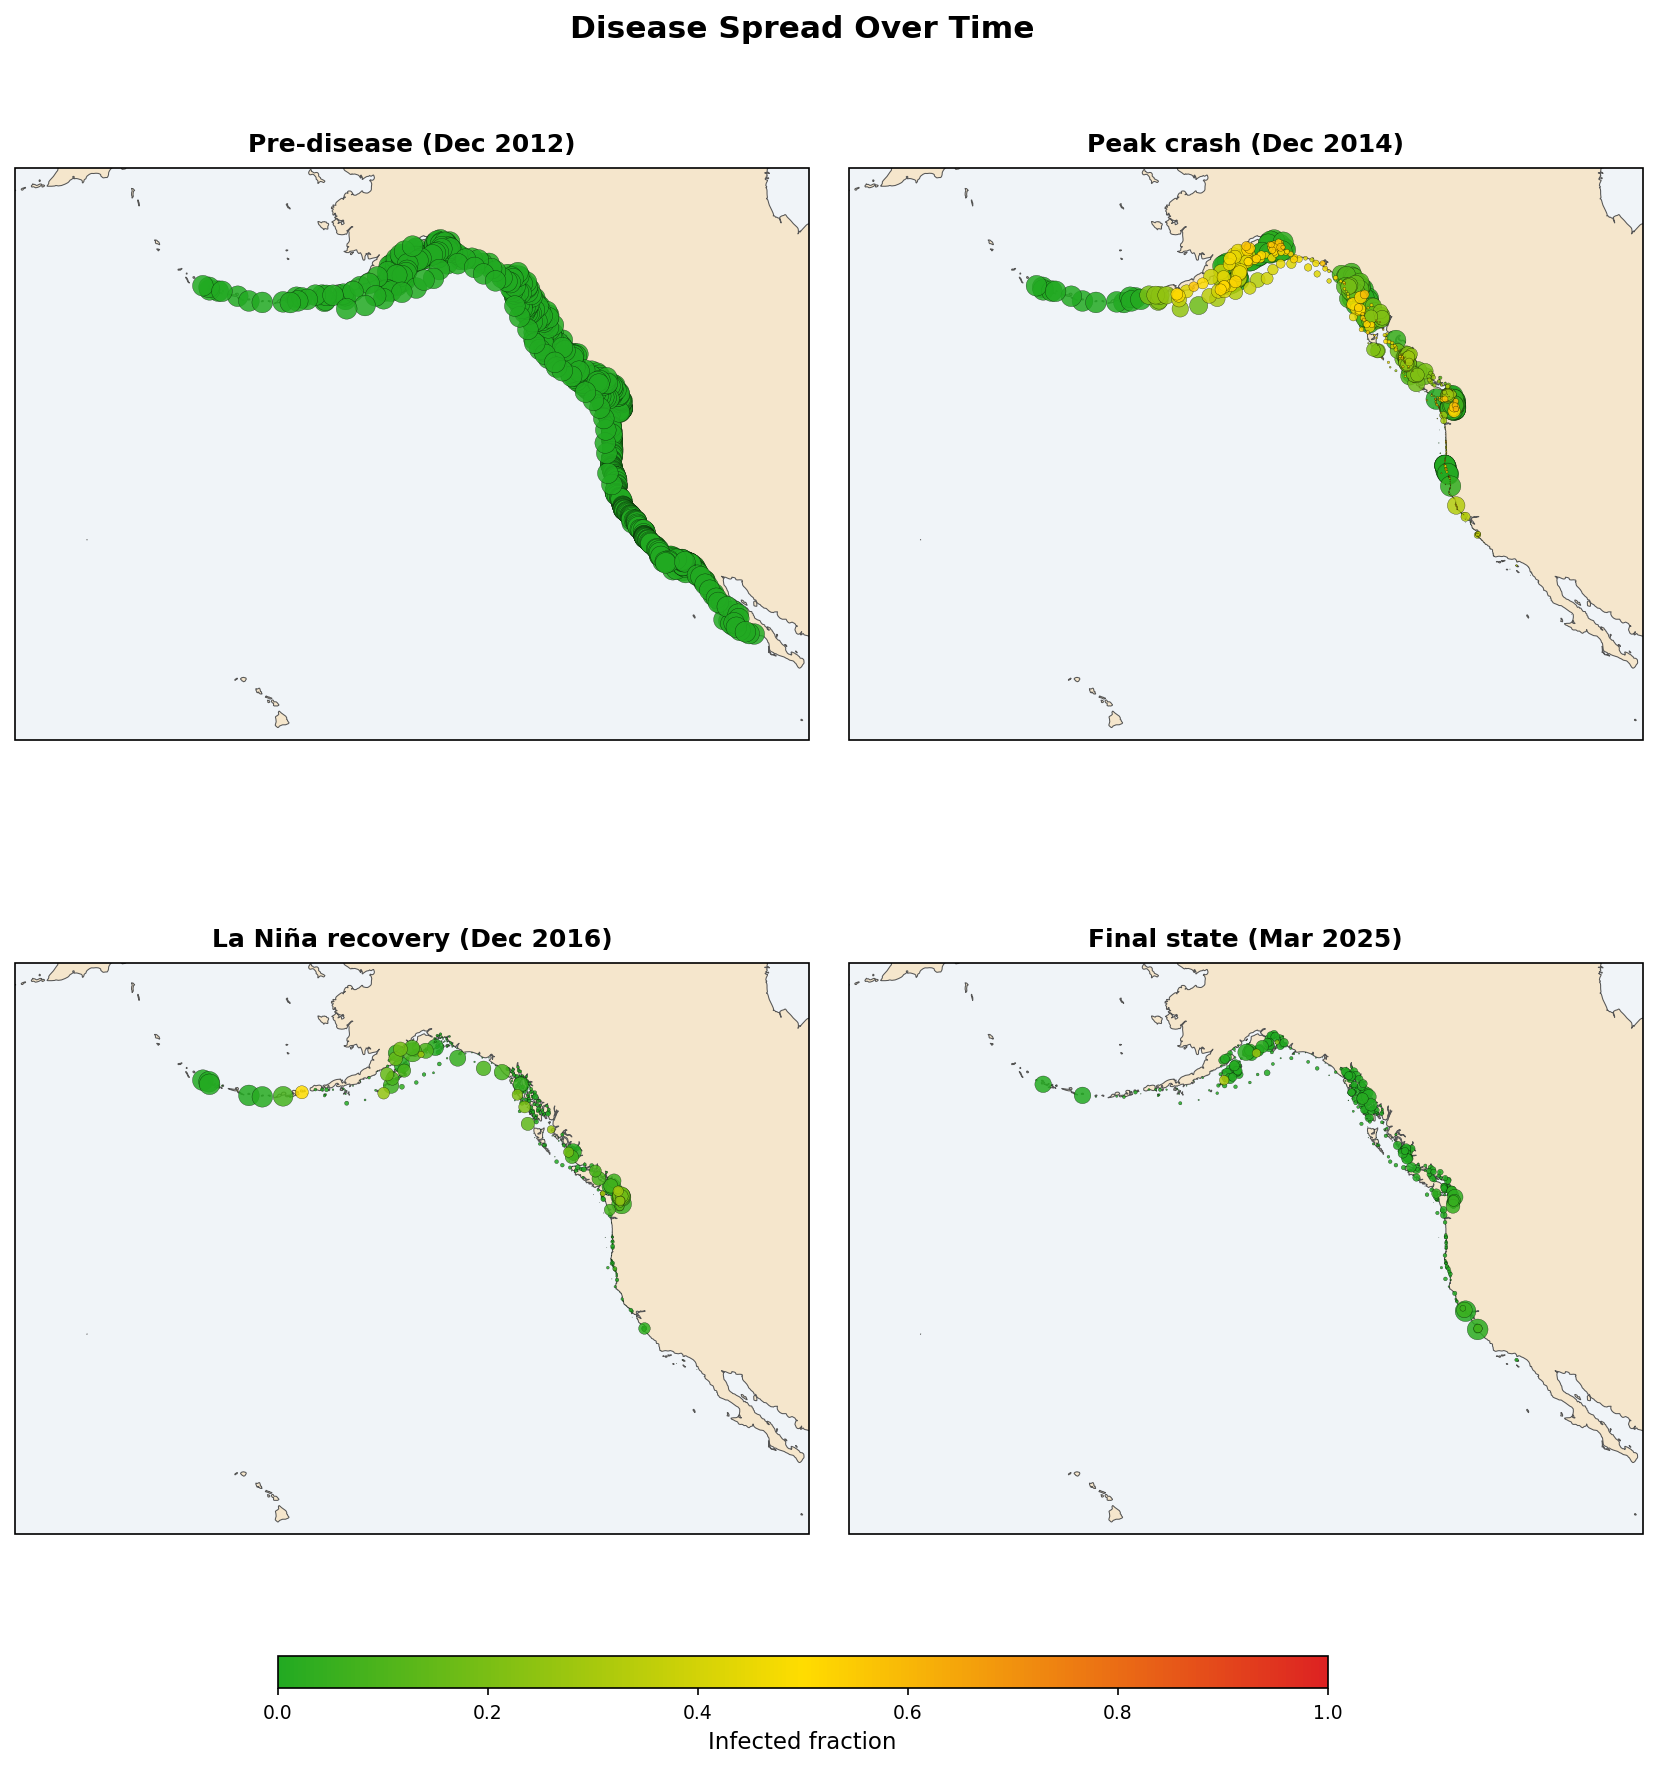
\includegraphics[width=0.95\textwidth]{figures/fig_disease_snapshots.png}
    \caption{Four snapshots of the disease simulation. \textbf{Top left:} Pre-disease (2012), all populations near carrying capacity. \textbf{Top right:} Peak crash (2014--2015), disease spreading northward from southern California. \textbf{Bottom left:} Mid-simulation (2016--2017), partial recovery in Alaska driven by seasonal pathogen dormancy and larval recruitment. \textbf{Bottom right:} Final state (2024), showing the persistent north--south gradient in population survival.}
    \label{fig:snapshots}
\end{figure}

The disease agent in our model is \textit{Vibrio pectenicida}, confirmed as a candidate SSWD pathogen by Prentice et al.\ (2025). Understanding one key aspect of \textit{Vibrio} biology is essential to understanding everything else in the model: the \textbf{VBNC state}.

\subsection*{The VBNC State: A Bacterial Survival Strategy}

VBNC stands for ``viable but non-culturable''---a well-documented survival state in many \textit{Vibrio} species \citep{liu2019}. As water temperatures drop, bacteria progressively shift into dormancy. We model this as a \textbf{sigmoid transition} centered at $T_{\text{vbnc}} = 12$\textdegree C (with steepness $k = 2.0$): at 14\textdegree C the pathogen is $\sim$98\% active, at 12\textdegree C it is 50\% active, and at 10\textdegree C only $\sim$2\% remain active. In VBNC dormancy, bacteria are alive but metabolically suppressed---they cannot cause disease, and they cannot be grown in laboratory cultures (hence ``non-culturable''). When temperatures rise again, the bacteria ``wake up'' and become infectious.

This has profound implications for SSWD dynamics along the Pacific coast:
\begin{itemize}[leftmargin=2em]
    \item In \textbf{southern California and Baja}, where water temperatures routinely exceed 12\textdegree C, the pathogen can remain active year-round. Disease pressure is relentless.
    \item In \textbf{Alaska}, where water temperatures may only briefly exceed 12\textdegree C during summer, the pathogen has a limited window of activity. Stars get a seasonal reprieve.
    \item We also set a \textbf{thermal adaptation floor} at $T_{\text{vbnc,min}} = 9$\textdegree C: the pathogen community cannot evolve its activation midpoint below this temperature. Even at the floor, the sigmoid means bacterial activity approaches zero asymptotically below 9\textdegree C rather than shutting off completely---but at $\sim$7\textdegree C, activity is negligible ($<$2\%). This floor is supported by laboratory studies of \textit{Vibrio} thermal limits, which show growth cessation below approximately 10\textdegree C.
\end{itemize}

\subsection*{How Disease Spreads: The Wavefront}

Based on observational data, SSWD appeared first in the Channel Islands (southern California) in mid-2013 and spread northward along the coast as a wave, reaching Alaska by 2014--2015. Our model reproduces this pattern through three mechanisms working together:

\begin{enumerate}[leftmargin=2em]
    \item \textbf{Thermal activation:} Disease can only establish at a site when local water temperature exceeds the VBNC threshold. Southern sites warm up first each year, so the disease front naturally progresses from south to north.

    \item \textbf{Cumulative pathogen dose:} A site does not become diseased instantly upon first pathogen arrival. Instead, pathogen units accumulate over time, and disease only ``ignites'' when the cumulative dose exceeds a threshold of 1,000 units. This creates a realistic lag between first exposure and outbreak onset.

    \item \textbf{Waterborne dispersal:} The pathogen travels between connected sites through the water, carried by currents. Sites closer together exchange more pathogen. This dispersal kernel allows the disease wave to propagate along the coast.
\end{enumerate}

\subsection*{The Environmental Pathogen Pool}

Each site in the model maintains an \textbf{environmental pathogen reservoir}---the total amount of \textit{Vibrio} in the water and sediment at that location. This reservoir is dynamic:

\begin{itemize}[leftmargin=2em]
    \item It \textbf{grows} when infected stars shed pathogen into the environment. Symptomatic (I$_2$) individuals are the dominant source, shedding at 10$\times$ the rate of pre-symptomatic (I$_1$) individuals. Dying stars also release a burst of bacteria, though the per-day contribution is smaller than active I$_2$ shedding. The parameter $\alpha_{\text{env}}$ controls what fraction of total shedding enters the persistent environmental pool.
    \item It \textbf{decays} naturally over time as bacteria die or are consumed by other microbes ($\delta_{\text{env}} = 0.02$ per day, giving a half-life of approximately 35 days).
    \item The probability that a healthy star becomes infected depends on the size of this reservoir relative to a half-saturation constant ($K_{\text{half}} = 800{,}000$), following Michaelis--Menten kinetics. When the reservoir equals $K_{\text{half}}$, the dose--response component is at 50\% of its maximum. The actual daily infection probability also depends on the individual's resistance, body size, and local salinity, so the effective infection rate at $K_{\text{half}}$ is typically 20--30\% for an average star. At lower pathogen levels, infection risk drops further; at higher levels, the dose--response saturates.
\end{itemize}

This density-dependent infection mechanism is biologically intuitive: the more pathogen in the water, the more likely a star is to encounter an infectious dose.

\section{Pathogen Community Evolution}

\begin{figure}[ht]
    \centering
    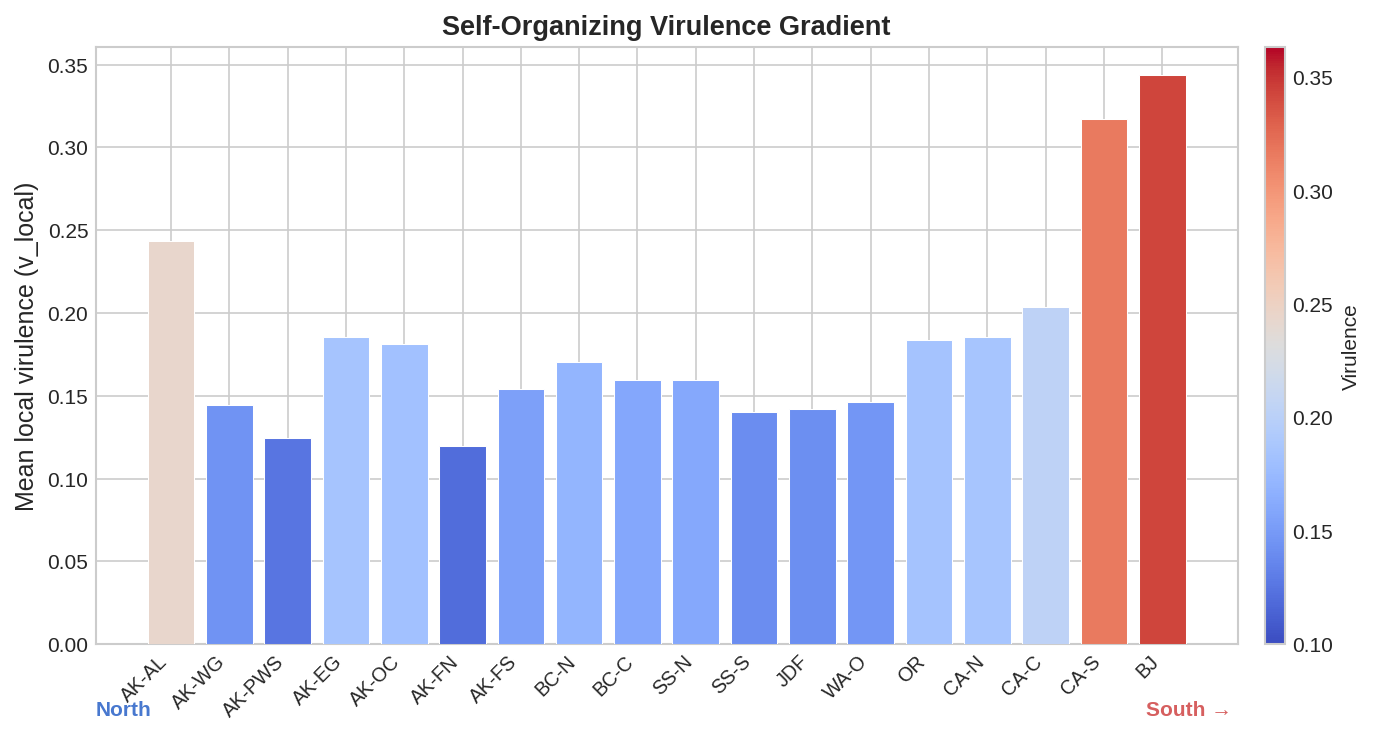
\includegraphics[width=0.75\textwidth]{figures/fig_virulence_gradient.png}
    \caption{Virulence gradient across the species' range. Warmer southern sites evolve higher virulence (more aggressive pathogen), while colder northern sites evolve lower virulence (more persistent pathogen). Each site's virulence drifts toward a local optimum determined by temperature and host density, producing a latitudinal gradient.}
    \label{fig:virulence}
\end{figure}

One of the most novel aspects of our model is that we allow the \textbf{pathogen community to evolve} at each site. This is based on a key conceptual insight: rather than tracking individual bacterial strains (which would be computationally prohibitive at this scale), we treat the bacterial community at each site as the evolutionary unit. The community has aggregate properties---like average virulence and thermal sensitivity---that shift over time in response to local selection pressures.

Each site's pathogen community has two evolving traits:

\begin{enumerate}[leftmargin=2em]
    \item \textbf{Thermal activation threshold ($T_{\text{vbnc}}$):} The temperature midpoint at which local bacteria transition from dormancy to activity (modeled as a sigmoid, not a hard cutoff). Over time, bacteria at cold-water sites evolve lower thresholds, allowing them to activate at cooler temperatures. Warm-water sites experience little change because the pathogen is already active year-round---there is no selection pressure for further cold-adaptation.

    \item \textbf{Local virulence ($v_{\text{local}}$):} How deadly the infection is. This trait evolves according to a classic idea in evolutionary biology: the \textbf{virulence--transmission trade-off} \citep{anderson1982}.
\end{enumerate}

The virulence--transmission trade-off works as follows. A more virulent pathogen kills its host faster, which in the short term releases a larger burst of pathogen into the environment (high transmission). But killing the host too quickly also means the host stops shedding pathogen sooner. The optimal strategy depends on the environment:

\begin{itemize}[leftmargin=2em]
    \item In \textbf{warm southern waters} where the pathogen is active year-round and encounters between hosts are frequent, \textbf{high virulence} is favored. Quick kill, massive pathogen release, plenty of new hosts available.
    \item In \textbf{cold northern waters} where the pathogen has a limited activity window, \textbf{lower virulence} is favored. Keeping the host alive longer means the host sheds pathogen throughout the brief warm season, maximizing total transmission.
\end{itemize}

We implement this trade-off phenomenologically: each site's pathogen community drifts toward a \textbf{local optimal virulence} determined by temperature and host density (Figure~\ref{fig:virulence}). The formula maps warm, high-density environments to higher optimal virulence and cold, sparse environments to lower optimal virulence, following the predictions of Anderson \& May. The resulting gradient---local virulence ranging from approximately 0.08 in Alaska to approximately 0.35 in Baja California---is thus \textit{shaped by} the underlying theory rather than discovered de novo by the model. However, the feedback between virulence, host mortality, and population density means the final gradient reflects genuine ecological dynamics: high virulence in the south depletes host populations, which in turn constrains how far virulence can rise.

The biological implication is striking: southern \textit{Pycnopodia} face a fundamentally more aggressive pathogen than their northern counterparts. But northern stars face a more persistent one---lower virulence means infections last longer, and the pathogen returns every warm season.

\subsection{Thermal Cold-Adaptation}

\begin{figure}[ht]
    \centering
    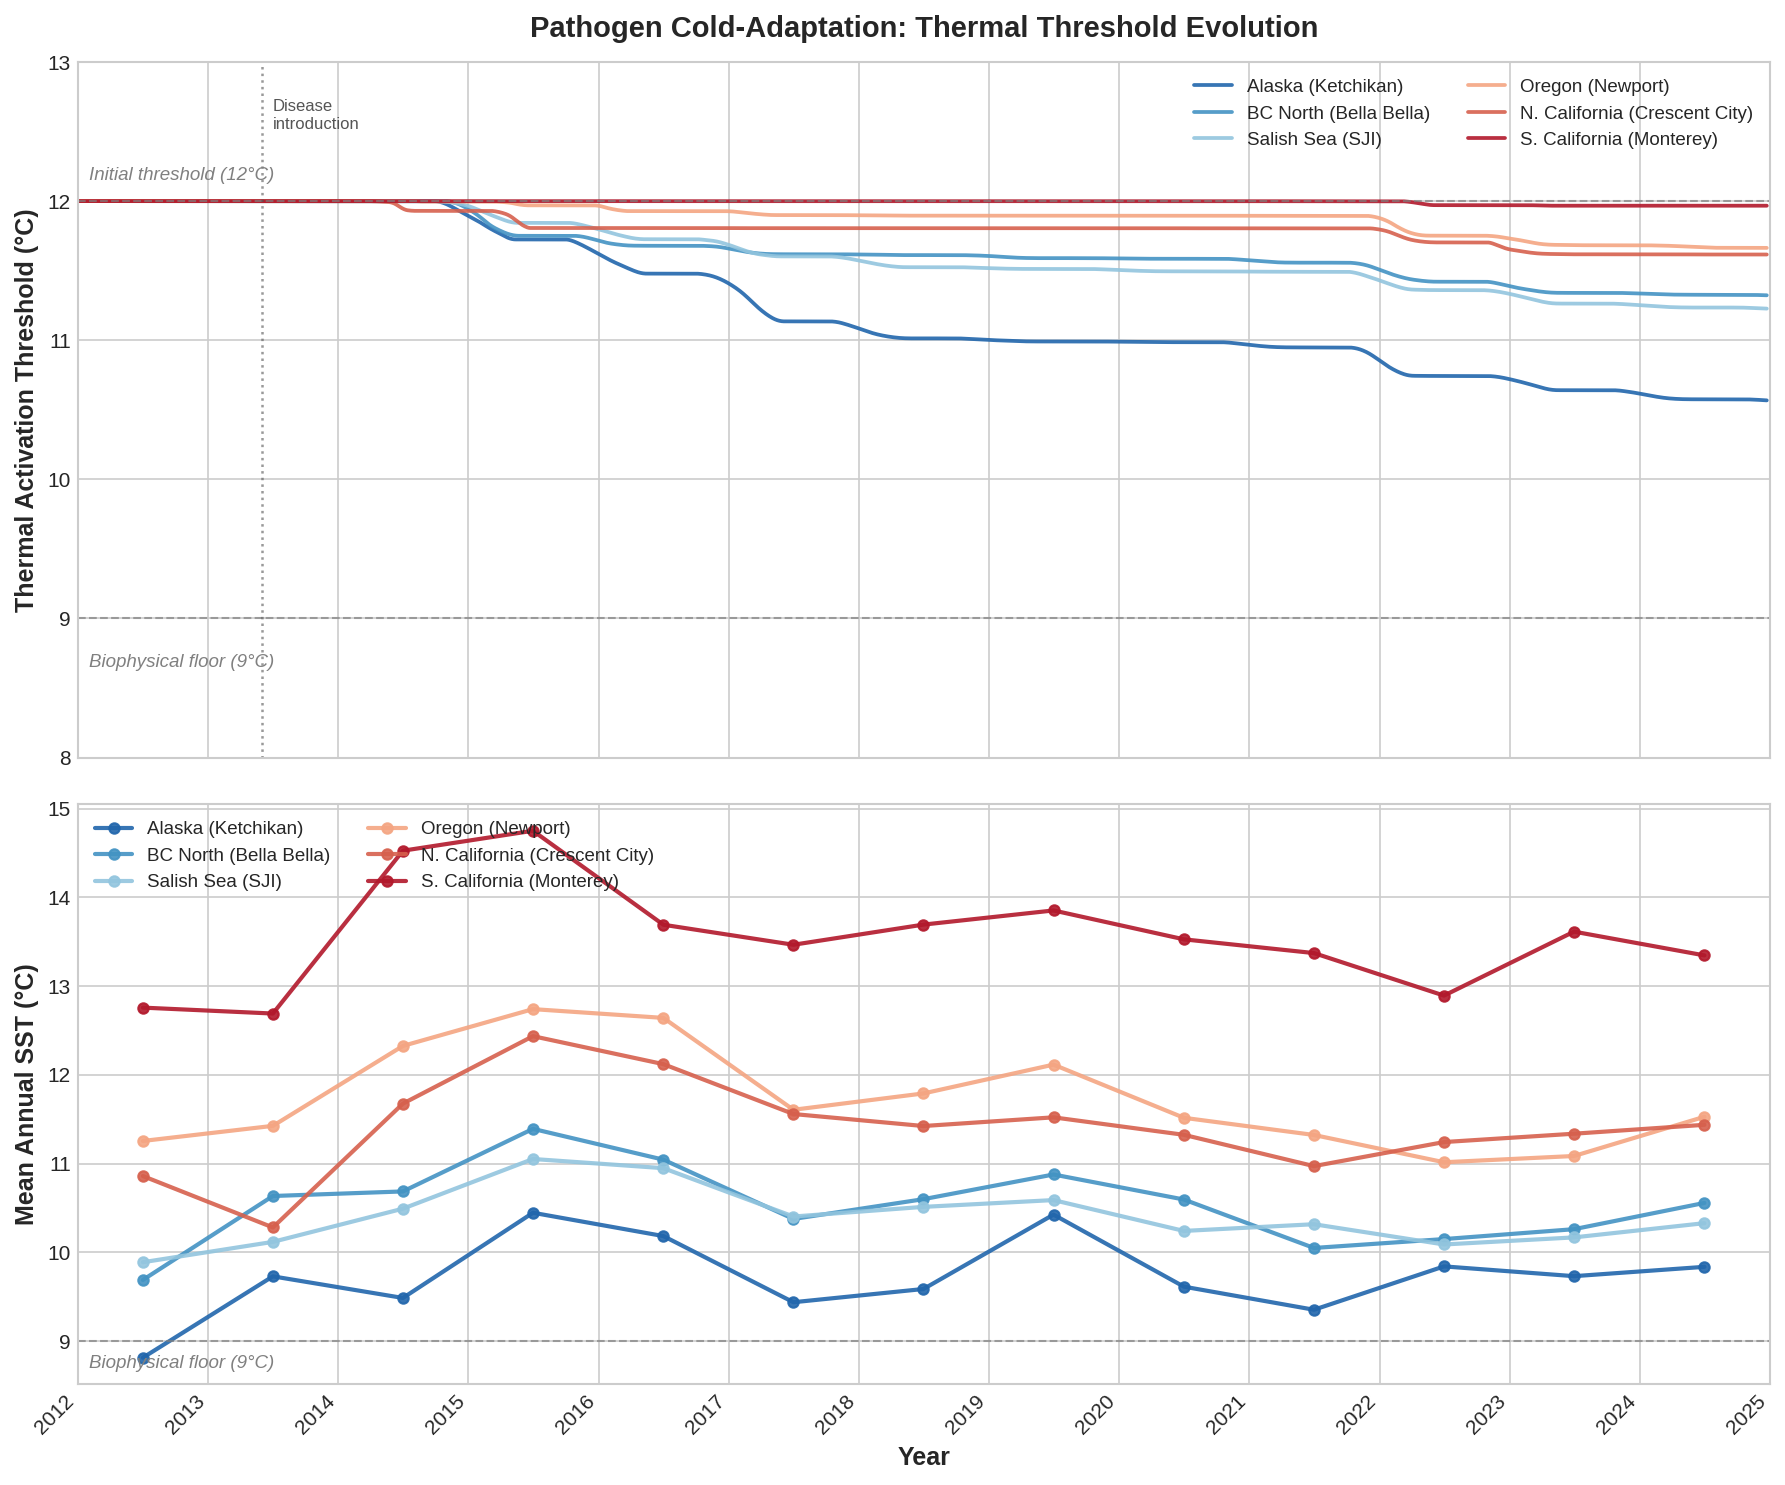
\includegraphics[width=0.95\textwidth]{figures/fig_thermal_adaptation.png}
    \caption{\textbf{Top:} Evolution of the pathogen thermal activation threshold ($T_{\text{vbnc,local}}$) over the 13-year simulation for six representative regions. All sites begin at 12\textdegree C. In cold northern waters (dark blue), the pathogen community rapidly adapts to activate at lower temperatures, driven by strong selection during winter months when SST falls well below the threshold. In warm southern waters (red), the pathogen is already active year-round and there is little selection pressure for cold-adaptation. The dashed line at 9\textdegree C marks the biophysical floor---the lowest temperature at which \textit{Vibrio} can feasibly transition from dormancy. \textbf{Bottom:} Mean annual sea surface temperature for each region, showing the thermal gradient that drives differential adaptation rates. Note that Alaska's mean SST hovers near the 9\textdegree C floor, explaining why its pathogen community evolves the furthest.}
    \label{fig:thermal}
\end{figure}

The second evolving trait---the thermal activation threshold---tells a complementary story (Figure~\ref{fig:thermal}). Each site's pathogen community begins with a threshold of 12\textdegree C, meaning bacteria transition from dormancy (VBNC state) to active growth only when water temperatures exceed this value. Over time, at sites where the pathogen is present but temperatures routinely fall below the threshold, the community's effective threshold drifts downward---a phenomenological approximation of how cold-tolerant strains would be favored in such environments.

Counter-intuitively, this means the \textbf{coldest sites show the greatest thermal adaptation}. In Alaska, where SST spends much of the year below 12\textdegree C, there is sustained selection pressure for bacteria that can activate at progressively lower temperatures. The pathogen community at Alaskan sites evolves its threshold down to approximately 10.5\textdegree C---extending its active season by several weeks. Meanwhile, at southern California sites where water temperatures rarely drop below 12\textdegree C, the threshold barely changes: there is simply no selection pressure for cold-adaptation when the environment is already warm enough for year-round activity.

This adaptation is bounded by a hard biophysical floor at 9\textdegree C, representing the lowest temperature at which \textit{Vibrio} can plausibly maintain metabolic activity. Below this point, the bacterium enters true dormancy regardless of any evolutionary pressure. The model treats this as an absolute constraint---no amount of selection can push a bacterial community to activate below 9\textdegree C.

The interplay between thermal adaptation and virulence evolution creates a nuanced picture of pathogen strategy across the range. Northern pathogen communities evolve to be \textit{more cold-tolerant but less virulent}---extending their active season while keeping hosts alive longer to maximize transmission during brief warm windows. Southern communities evolve to be \textit{already warm-adapted but highly virulent}---exploiting year-round activity with an aggressive kill-and-spread strategy. While these two traits evolve via separate phenomenological rules in the model, both are driven by the same underlying thermal gradient, producing correlated patterns that are consistent with theoretical predictions for pathogen life-history optimization.

\subsection{Evolutionary Divergence Across Regions}

\begin{figure}[ht]
    \centering
    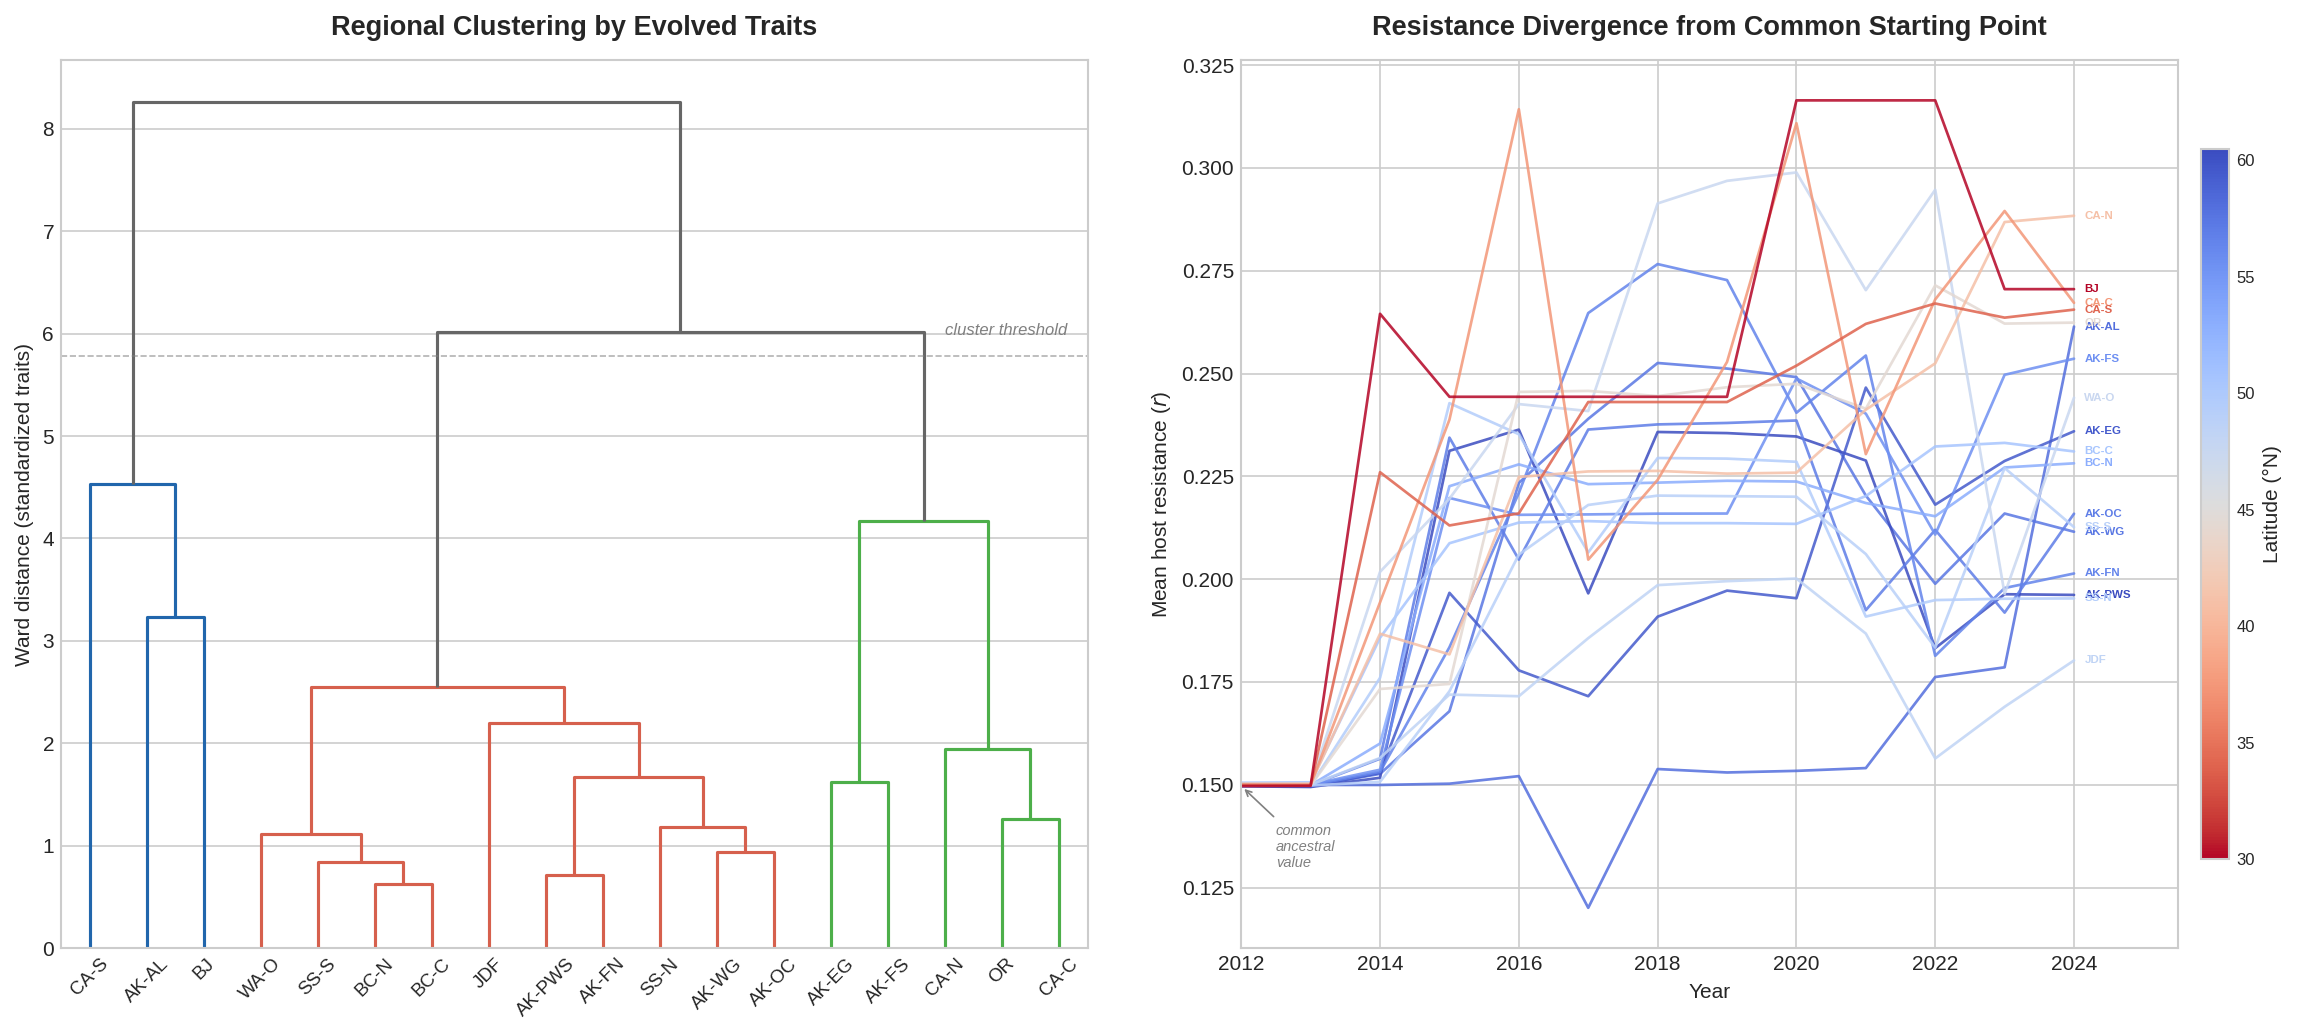
\includegraphics[width=0.95\textwidth]{figures/fig_evolution_dendrogram.png}
    \caption{\textbf{Left:} Hierarchical clustering (dendrogram) of the 18 regions based on their final evolved trait profiles (host resistance, tolerance, recovery, pathogen thermal threshold, and virulence). Regions that cluster together evolved similar phenotypes by the end of the simulation. \textbf{Right:} Divergence of mean host resistance over time. All regions begin at $r \approx 0.15$; southern regions (red tones) are driven to higher resistance under intense disease pressure, while northern regions (blue tones) evolve more slowly. The fan-like divergence pattern reflects how a single initial gene pool can be pulled apart by spatially varying selection.}
    \label{fig:dendrogram}
\end{figure}

When we examine the final evolved state across all 18 regions, a striking pattern of \textbf{regional clustering} emerges (Figure~\ref{fig:dendrogram}, left). By computing the similarity of each region's final trait profile---considering host resistance, tolerance, recovery, pathogen thermal threshold, and virulence together---we can group regions that arrived at similar evolutionary endpoints. Northern Alaskan regions cluster tightly (moderate resistance, low pathogen virulence, preserved genetic diversity), while southern regions form a distinct cluster (high resistance, high virulence, depleted diversity).

The right panel of Figure~\ref{fig:dendrogram} tells this story dynamically. Every region starts from the same place---mean resistance $r \approx 0.15$---but they diverge over the 13-year simulation like branches from a common trunk. Southern populations are pushed hardest (stronger disease selection) and evolve the fastest, while northern populations drift more gradually. This is analogous to an adaptive radiation, where a single ancestral population splits into distinct ecotypes under different environmental pressures---except here it happens within a single decade under epidemic selection.

\section{Temperature-Driven Population Dynamics}

\begin{figure}[ht]
    \centering
    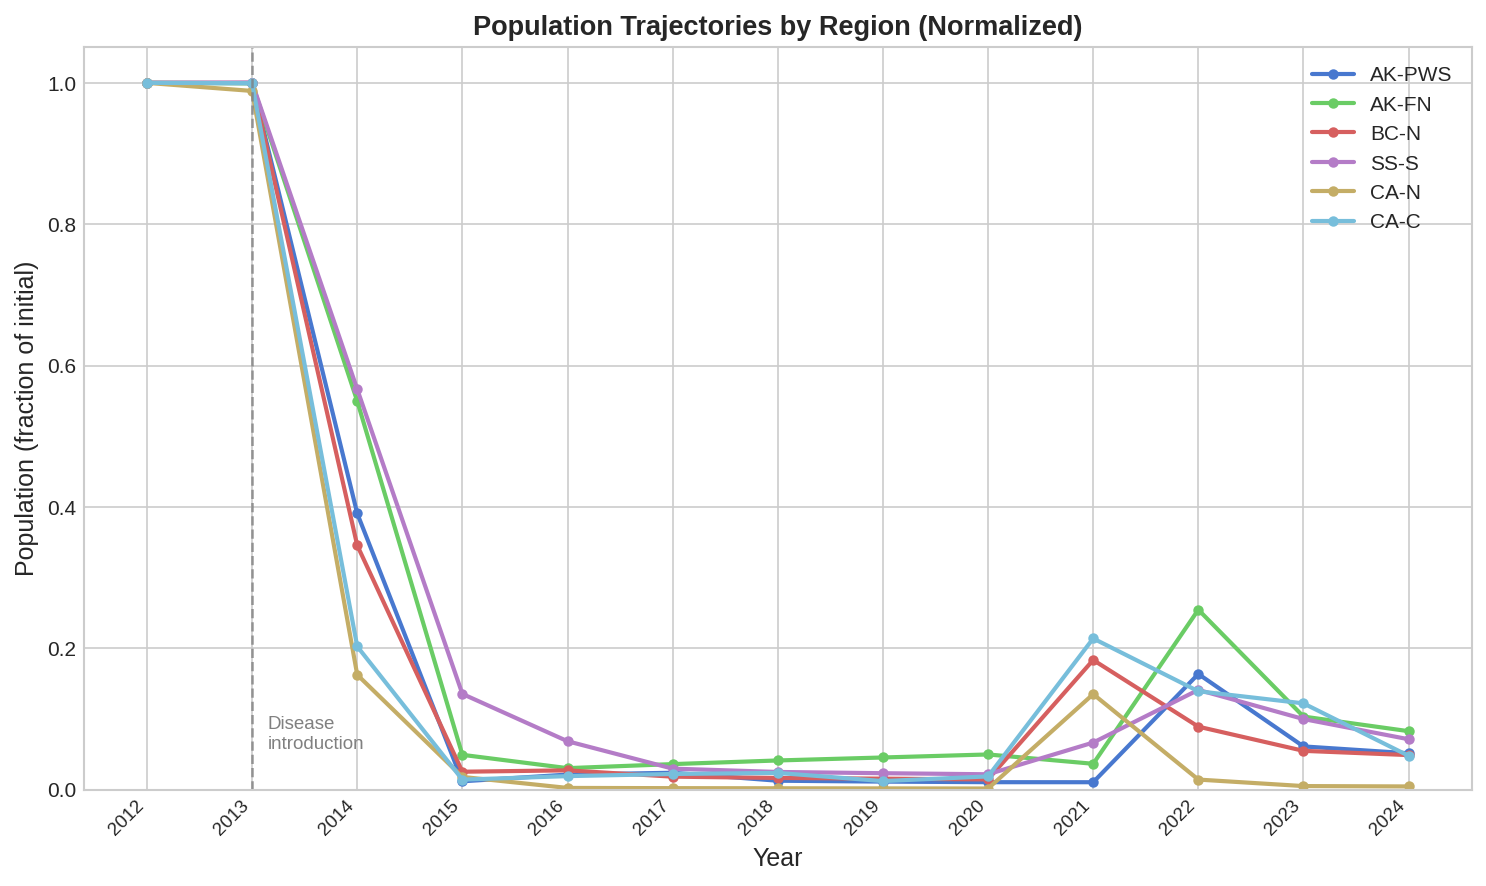
\includegraphics[width=0.85\textwidth]{figures/fig_population_trajectories.png}
    \caption{Normalized population trajectories for selected regions over the 13-year simulation. Note the recovery spikes in Alaska populations (blue tones), driven primarily by larval recruitment pulses from neighboring sites with surviving populations, combined with seasonal windows of reduced pathogen activity during cold months.}
    \label{fig:trajectories}
\end{figure}

\begin{figure}[ht]
    \centering
    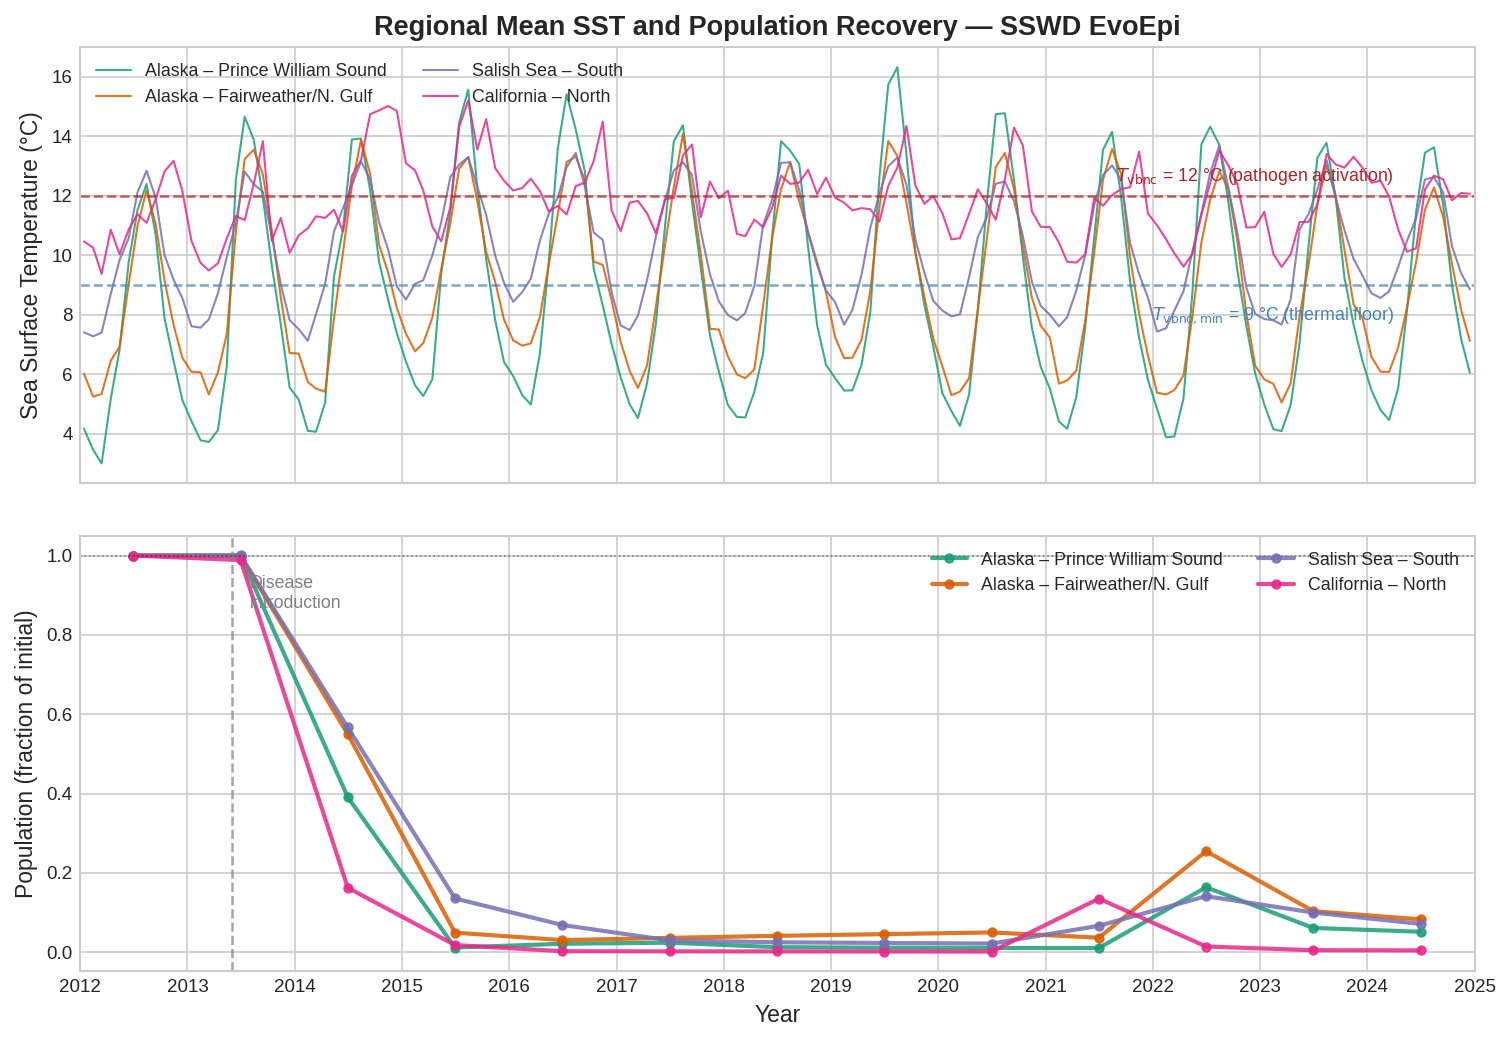
\includegraphics[width=0.95\textwidth]{figures/fig_sst_recovery.png}
    \caption{Sea surface temperature (top) and population dynamics (bottom) for four key regions. The horizontal dashed lines in the top panel mark the pathogen activation temperature ($T_\text{vbnc} = 12$\textdegree C) and thermal adaptation floor ($T_\text{vbnc,min} = 9$\textdegree C, below which bacteria remain dormant but persist). Note the strong seasonal SST cycles in Alaska, which drive annual VBNC cycling and create narrow windows of disease activity.}
    \label{fig:sst_recovery}
\end{figure}

One of the most interesting features of the model is the \textbf{interplay between temperature cycles and population dynamics}. Because the model uses real satellite SST data, it captures climate variability---including ENSO events like La Ni\~na---without any explicit programming.

After the initial disease crash (2013--2015), Alaska populations remain severely depleted for several years before showing a dramatic \textbf{recruitment pulse around 2021--2022} (Figures~\ref{fig:trajectories} and \ref{fig:sst_recovery}). In AK-PWS, the population surges from $\sim$2,200 to $\sim$34,800 in a single year, driven by over 71,000 recruits---far more than could be produced by the local survivors alone. This pulse is primarily fueled by \textbf{larval import} from neighboring sites with slightly larger surviving populations, reflecting the spatial connectivity built into the model.

Importantly, this recovery pulse is \textbf{not stable}. Disease deaths immediately surge in the following year ($\sim$19,700 in 2023), driving the population back down. The fundamental problem remains: the pathogen reactivates every warm season, and resistance has not evolved far enough to provide lasting protection.

The SST data (Figure~\ref{fig:sst_recovery}) reveals why Alaska's thermal environment is so challenging for recovery. Alaska SST oscillates around the 12\textdegree C pathogen activation threshold on an annual cycle, creating a recurring \textbf{warm-season disease window}. During winter, bacteria enter VBNC dormancy and disease pressure drops, allowing some reproduction. But every summer, the pathogen reactivates and new infections sweep through the population. The model captures this seasonal ratchet naturally from the temperature data.

This has a practical implication: \textbf{observed population fluctuations in Alaska field surveys likely reflect this seasonal disease cycling rather than true recovery}. A population that grows during winter and crashes each summer may appear to be recovering when surveyed in spring, but this does not indicate a sustained trajectory toward pre-disease levels.

\section{Calibration Targets}

The model was calibrated against two types of empirical observations:

\subsection*{Disease Arrival Timing}
The historical record tells us when SSWD arrived in each region. Disease was first documented in the Channel Islands (southern California) in June 2013, then spread northward---reaching Oregon by late 2014, the Salish Sea by early 2015, and Alaska by mid-2015 to 2016. We use 17 regional arrival time targets (in months after the initial outbreak) to ensure the model's wavefront spreads at a realistic speed.

\subsection*{Recovery Targets}
Our primary calibration metric is the \textbf{fractional population recovery} at each region by the end of the simulation (2024), expressed as a percentage of pre-disease carrying capacity. These targets are based on the best available survey data and expert estimates:

\begin{center}
\small
\begin{tabular}{lrp{7.5cm}}
\hline
\textbf{Region} & \textbf{Target} & \textbf{Rationale} \\
\hline
AK-PWS (Prince William Sound) & 50\% & Substantial recovery documented in surveys; cold water limits disease activity \\
AK-FN (Fairweather North) & 50\% & Similar to PWS; remote cold-water populations \\
AK-FS (Fairweather South) & 20\% & Partial recovery; warmer than PWS \\
BC-N (British Columbia North) & 20\% & Moderate recovery in fjord-rich coast \\
SS-S (Salish Sea South) & 5\% & Limited recovery in semi-enclosed temperate waters \\
JDF (Juan de Fuca Strait) & 2\% & Near-total loss; exposed to warm summer waters \\
OR (Oregon) & 0.25\% & Severe decline with minimal recovery \\
CA-N (California North) & 0.1\% & Near-extirpation; warm year-round \\
\hline
\end{tabular}
\end{center}

The key pattern is a strong \textbf{latitudinal gradient}: northern populations (cold water, limited pathogen activity) retain or recover more individuals than southern populations (warm water, year-round pathogen activity). The model must reproduce this gradient---not just the absolute numbers, but the relative ordering---while also matching the wavefront timing.

We quantify the overall fit using \textbf{log-RMSE}: the root-mean-square error of the log-transformed target vs.\ actual recovery fractions. This metric weights relative errors equally across regions (a 10$\times$ overshoot at 0.1\% is penalized the same as a 10$\times$ overshoot at 50\%), which is appropriate given the four-order-of-magnitude range of the targets.

\section{Current Best Model Results}

\begin{figure}[ht]
    \centering
    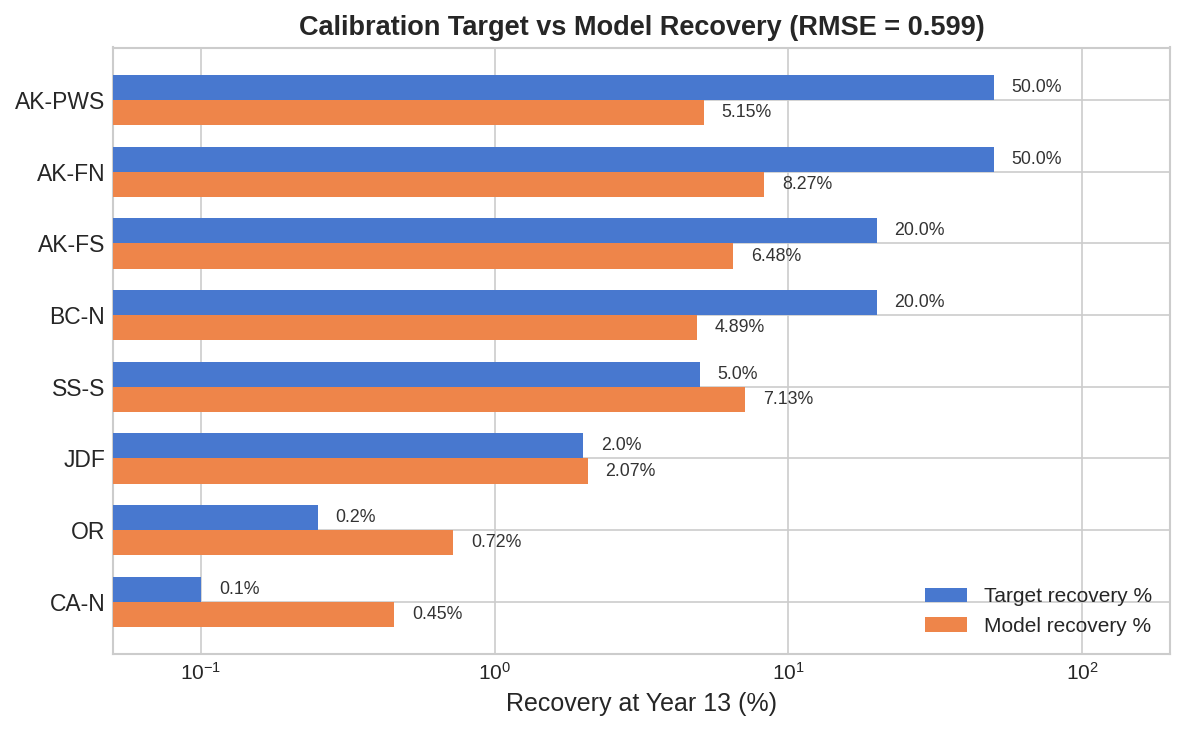
\includegraphics[width=0.85\textwidth]{figures/fig_recovery_comparison.png}
    \caption{Comparison of target (observed) vs.\ modeled population recovery by region (as percentage of pre-disease carrying capacity). The model accurately captures the near-total loss in southern regions and partial survival in mid-range regions, but underestimates recovery in Alaska.}
    \label{fig:recovery}
\end{figure}

Our best-performing parameter configuration to date is \textbf{W154}, which achieves a mean root-mean-square error (RMSE) of 0.504 across three independent simulation runs (best single seed: 0.479). In plain terms, the RMSE measures how far off the model's predictions are from observed recovery data---lower is better, and 0.599 represents a reasonable fit given the complexity of the system.

The key model settings, in biological terms:
\begin{itemize}[leftmargin=2em]
    \item Disease originates from 5 sites in the Channel Islands (southern California) in 2013, spreading northward as a wave
    \item The pathogen activates above 12\textdegree C and enters deep dormancy below 9\textdegree C (persists but cannot evolve to activate at lower temperatures)
    \item Bacterial communities evolve locally, adapting their thermal thresholds and virulence to match local conditions
    \item Host resistance starts at 15\% and evolves under natural selection
    \item Enclosed waterways retain both larvae (helpful) and pathogen (harmful)
    \item Site flushing rates are derived from an enclosedness metric, with a nonlinear mapping exponent ($n_{\text{conn}} = 0.3$)
\end{itemize}

\subsection*{What the Model Gets Right}

\begin{itemize}[leftmargin=2em]
    \item \textbf{Southern die-off:} CA-S and Baja California drop to $\sim$0\% of pre-disease levels, matching the observed near-total wipeout
    \item \textbf{Mid-range partial survival:} Juan de Fuca Strait shows 2.1\% recovery vs.\ a 2\% target (essentially perfect); Salish Sea South shows 7.1\% vs.\ a 5\% target (close)
    \item \textbf{North--south gradient:} The model correctly produces higher survival in the north and lower in the south
    \item \textbf{Virulence gradient:} The pathogen virulence pattern differentiates across the range, consistent with Anderson \& May trade-off theory
    \item \textbf{Temporal dynamics:} The wavefront speed, seasonal cycling, and recruitment pulses all arise from the model's mechanisms interacting with real SST data
\end{itemize}

\subsection*{What the Model Struggles With}

The main remaining challenge is \textbf{Alaska} (Figure~\ref{fig:recovery}). The model predicts 5.1\% recovery for Prince William Sound and 8.3\% for False North, but field observations suggest approximately 50\% recovery in these regions. Getting Alaska to recover sufficiently while keeping the southern populations at near-zero is the central calibration challenge.

We are actively working on this. A recent test with a higher half-saturation constant ($K_{\text{half}} = 1.2$ million, up from 800,000) dramatically lifts Alaska recovery---intuitively, requiring more pathogen in the water before infection kicks in gives cold-water populations more breathing room. However, this change also overshoots recovery in some southern regions. The next calibration round will combine the higher $K_{\text{half}}$ with stronger environmental pathogen suppression in warm waters to maintain the north--south gradient.

\section{Creative Process and AI-Assisted Modeling}

This is the second major iteration of the SSWD-EvoEpi model. The first attempt used a different computational architecture and was ultimately set aside in favor of the current design-first approach, where biological mechanisms were specified in detail before any code was written.

The model has gone through \textbf{154 calibration rounds} (designated W001 through W154), each testing different combinations of parameter values. This iterative process has been essential for understanding which mechanisms matter most and how they interact.

An unusual feature of this project is the role of the AI research assistant (Anton), who manages simulation runs on a dedicated computing server, analyzes results, identifies patterns, and proposes the next set of experiments to test. This human--AI collaboration allows us to explore the parameter space much more efficiently than would be possible manually.

The model's complexity grew incrementally as we discovered what was needed. We started with simple disease spread, then added the wavefront mechanism when we realized uniform spread could not produce the observed temporal pattern. We added VBNC dynamics when temperature dependence proved essential. Pathogen evolution was added to explain regional differences in disease severity. Enclosedness was added to capture the unique dynamics of fjords and inland seas. Each addition was grounded in published literature and motivated by specific model--data mismatches.

\section{Implications for Captive Breeding: Finding Super-Resistant Individuals}

\begin{figure}[ht]
    \centering
    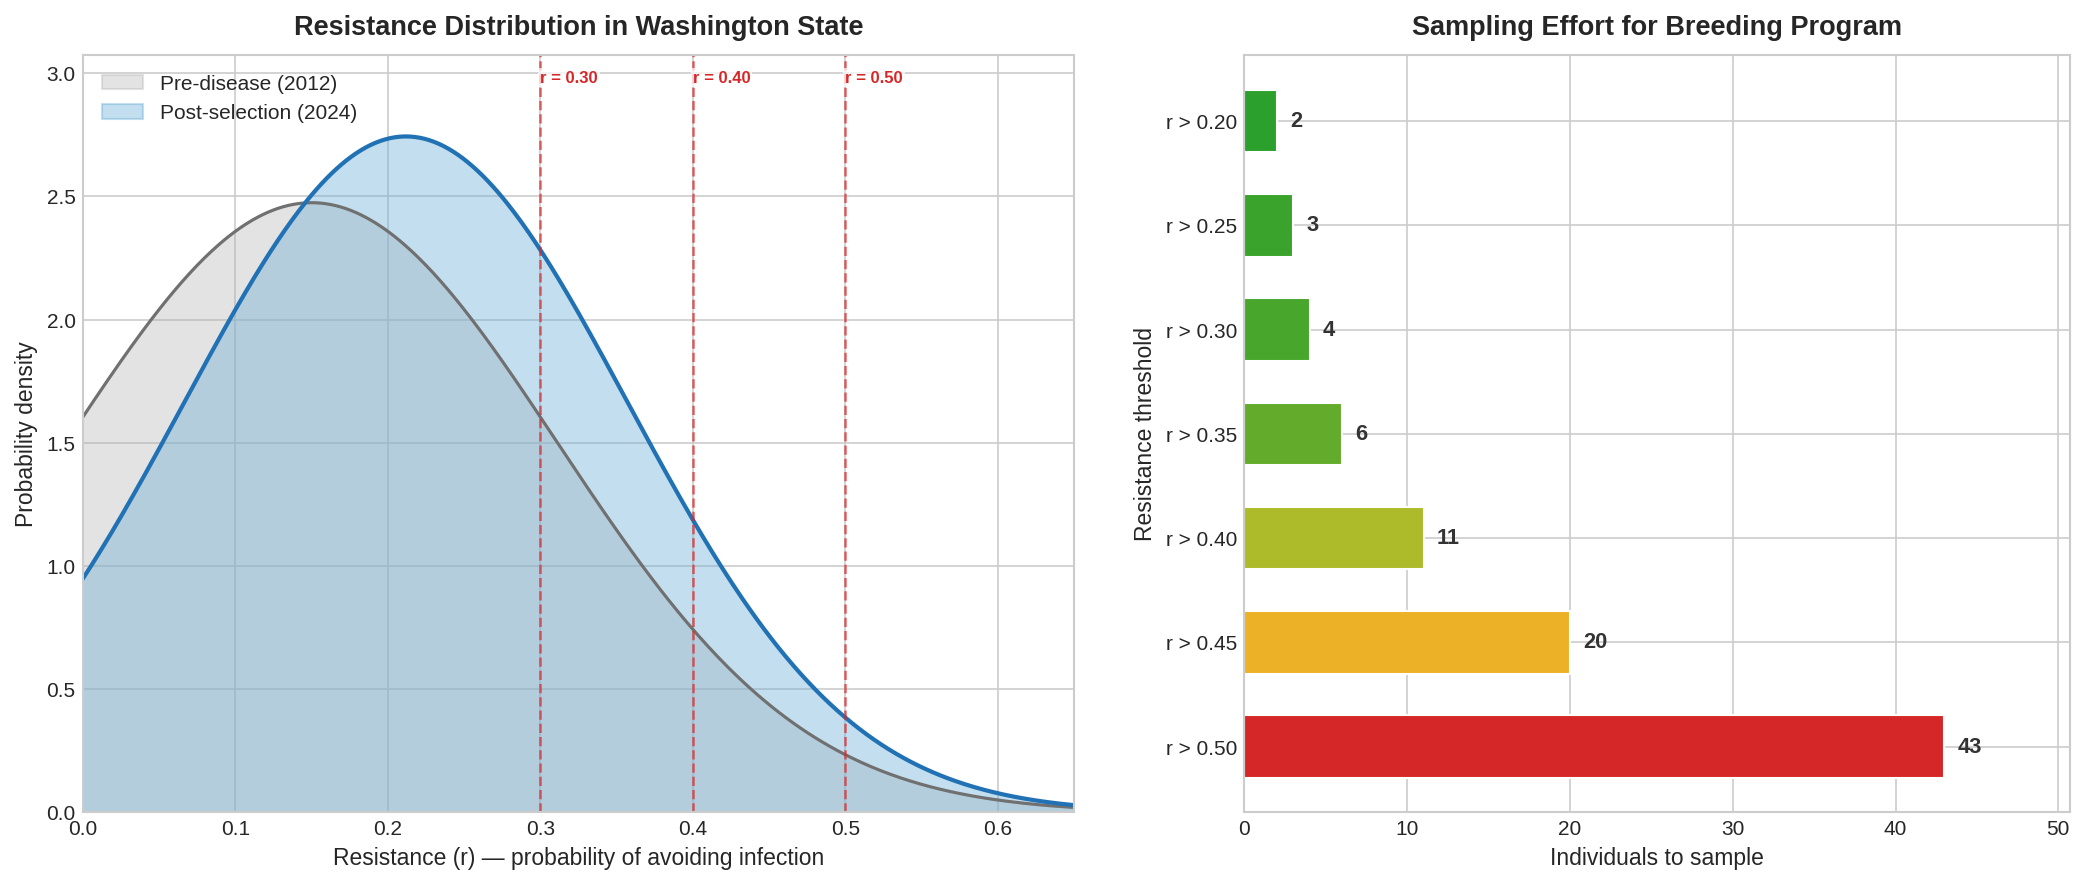
\includegraphics[width=0.95\textwidth]{figures/fig_breeding_sampling.png}
    \caption{\textbf{Left:} Distribution of host resistance in Washington State populations before (gray) and after (blue) 13 years of disease-driven selection. The post-selection distribution has shifted rightward (higher mean resistance) and the tail extends further. Vertical lines mark key resistance thresholds. \textbf{Right:} Number of wild individuals that would need to be sampled to find at least one individual exceeding each resistance threshold, based on the current genetic distribution.}
    \label{fig:breeding}
\end{figure}

A central motivation for this model is informing captive breeding and reintroduction strategies. One practical question is: \textbf{how many wild individuals would you need to collect from Washington State sites to find ``super-resistant'' broodstock?}

We can answer this from the model's genetic data. After 13 years of disease-driven selection, the Washington State populations (Salish Sea North and South, Juan de Fuca, outer Washington coast) have a pooled mean resistance of $\bar{r} = 0.21$ (up from the pre-disease 0.15) with a standard deviation of approximately 0.145. Assuming a roughly normal trait distribution (reasonable given the 17-locus additive architecture), we can compute the probability of finding individuals above any resistance threshold (Figure~\ref{fig:breeding}).

The results are encouraging for a breeding program:
\begin{center}
\small
\begin{tabular}{rrrl}
\hline
\textbf{Resistance} & \textbf{Hazard} & \textbf{Individuals} & \textbf{Interpretation} \\
\textbf{threshold} & \textbf{reduction} & \textbf{to sample} & \\
\hline
$r > 0.20$ & 20\% & 2 & Roughly half the population \\
$r > 0.30$ & 30\% & 4 & Still common \\
$r > 0.40$ & 40\% & 11 & Rare but findable \\
$r > 0.50$ & 50\% & 43 & Requires dedicated screening \\
\hline
\end{tabular}
\end{center}

To find an individual with $r > 0.50$ (a 50\% reduction in infection hazard---roughly halving the instantaneous risk per pathogen encounter), you would need to screen approximately \textbf{43 individuals}. This is logistically feasible for a well-resourced breeding program. For more modest thresholds ($r > 0.30$, meaning a 30\% hazard reduction---still significantly better than population average), you only need about 4 individuals.

Several important caveats apply:

\begin{itemize}[leftmargin=2em]
    \item \textbf{Resistance is not directly measurable in the field} --- you cannot read an individual's $r$ value from its appearance. A screening program would need to use controlled pathogen exposure trials (challenge experiments) to identify resistant individuals, or develop genetic markers from the resistance-associated loci.
    \item \textbf{These estimates assume the model's genetic architecture is correct.} Our 17-locus additive model is inspired by \textit{Pisaster ochraceus} GWAS data; the true genetic basis of SSWD resistance in \textit{Pycnopodia} may differ.
    \item \textbf{Even $r = 0.50$ is not immunity.} A 50\% reduction in infection hazard still leaves these ``super-resistant'' individuals highly vulnerable in high-pathogen environments (daily infection probability can still exceed 20\%). Resistance buys time for reproduction, not invulnerability.
    \item \textbf{Selection has already occurred.} The 43,000 surviving stars in Washington represent the survivors of intense selection. These populations are \textit{enriched} for resistance alleles compared to pre-disease populations, making the current window a particularly good time to collect broodstock.
\end{itemize}

\section{Next Steps}

Several priorities remain for the near term:

\begin{enumerate}[leftmargin=2em]
    \item \textbf{Solve the Alaska recovery problem.} Fine-tuning the balance between $K_{\text{half}}$ and environmental pathogen dynamics ($\alpha_{\text{env}}$, $\delta_{\text{env}}$) to achieve realistic Alaska recovery without compromising the southern die-off.

    \item \textbf{Sensitivity analysis.} We plan to run Morris screening and Sobol variance-based sensitivity analyses to systematically determine which parameters the model is most sensitive to. This will guide future calibration and tell us where our uncertainty matters most.

    \item \textbf{Reintroduction scenario modeling.} This is the ultimate goal of the project. Once the model reliably reproduces historical disease dynamics, we will use it to simulate captive breeding release strategies---testing different release locations, numbers, timing, and genetic compositions to identify the approaches most likely to establish self-sustaining populations.

    \item \textbf{Publication.} Preparing the model and its results for peer-reviewed publication.

    \item \textbf{Spatial snapshot recorder.} Adding an optional recorder that dumps individual agent positions at configurable intervals during model runs. This would allow visualization of within-site spatial dynamics from actual production runs (including effects of larval import, inter-site pathogen dispersal, and genetic evolution), but is deferred due to the I/O and memory overhead it would impose on large-scale calibration sweeps.
\end{enumerate}

\section*{Acknowledgments}

We thank the members of the Hodin Lab and the broader \textit{Pycnopodia} research community for ongoing discussions. SST data were provided by NOAA OISST. Computing resources were provided by a dedicated Xeon server.

\bibliographystyle{plainnat}

\clearpage
\section*{Appendix: Model Parameters}

The following tables list all model parameters grouped by category. Values shown are those used in the W142 configuration unless noted otherwise. Parameters marked with $\dagger$ were actively varied during calibration.

\small
\begin{longtable}{p{3.5cm} p{1.5cm} p{1.5cm} p{6.5cm}}
\hline
\textbf{Parameter} & \textbf{Symbol} & \textbf{Value} & \textbf{Description} \\
\hline
\endfirsthead
\hline
\textbf{Parameter} & \textbf{Symbol} & \textbf{Value} & \textbf{Description} \\
\hline
\endhead
\hline
\endfoot

\multicolumn{4}{l}{\textbf{Disease Transmission}} \\
\hline
Exposure coefficient & $a_\text{exp}$ & 0.75 & How efficiently pathogen in the environment translates to infection risk per exposure event \\
Half-saturation constant$^\dagger$ & $K_\text{half}$ & 800,000 & Amount of environmental pathogen needed for 50\% infection probability. Higher values = harder to get infected \\
Pathogen activation temp & $T_\text{vbnc}$ & 12\textdegree C & Temperature above which dormant \textit{Vibrio} become infectious \\
VBNC sigmoid steepness & $k_\text{vbnc}$ & 2.0 & How sharply the transition from dormant to active occurs around $T_\text{vbnc}$ \\
Thermal adaptation floor & $T_\text{vbnc,min}$ & 9\textdegree C & Lowest temperature the pathogen can evolve to activate at. Below this, bacteria remain dormant but persist \\
\hline

\multicolumn{4}{l}{\textbf{Environmental Pathogen Pool}} \\
\hline
Background Vibrio input & $P_\text{env,max}$ & 2,000 & Maximum background environmental \textit{Vibrio} production rate (bact/mL/d), modulated by VBNC activation and salinity \\
Accumulation rate$^\dagger$ & $\alpha_\text{env}$ & 0.18 & Fraction of total host shedding that enters the persistent environmental pool \\
Decay rate & $\delta_\text{env}$ & 0.02 & Daily fraction of environmental pathogen that degrades (2\%/day) \\
Pool floor & $P_\text{floor}$ & 500 & Minimum pathogen level maintained at active sites \\
\hline

\multicolumn{4}{l}{\textbf{Wavefront Disease Spread}} \\
\hline
Origin sites & --- & 5 & Channel Islands --- where SSWD was first documented in 2013 \\
Dose threshold & CDT & 1,000 & Cumulative pathogen exposure before local outbreak begins \\
Dispersal range & $D_P$ & 300 km & Characteristic distance waterborne pathogen travels between sites \\
Max dispersal & $D_{P,\text{max}}$ & 3,000 km & Maximum long-range pathogen dispersal distance \\
\hline

\multicolumn{4}{l}{\textbf{Disease Progression (within host)}} \\
\hline
Early shedding & $\sigma_1$ & 5.0 & Pathogen shed rate during pre-symptomatic stage \\
Late shedding & $\sigma_2$ & 50.0 & Pathogen shed rate during symptomatic stage (10$\times$ higher) \\
Death shedding & $\sigma_D$ & 15.0 & Pathogen burst released when an infected star dies \\
E$\to$I1 rate & $\mu_{EI1}$ & 0.233/d & Exposed to pre-symptomatic (at 20\textdegree C reference) \\
I1$\to$I2 rate & $\mu_{I1I2}$ & 0.434/d & Pre-symptomatic to symptomatic \\
I2$\to$Death rate & $\mu_{I2D}$ & 0.563/d & Symptomatic to death \\
Recovery rate & $\rho_\text{rec}$ & 0.05 & Base daily probability of clearing infection ($\times$ individual $c$ trait) \\
\hline

\multicolumn{4}{l}{\textbf{Pathogen Evolution}} \\
\hline
Thermal adapt rate & --- & 0.001/d & Speed at which local pathogen adapts its activation temperature \\
Virulence adapt rate & --- & 0.001/d & Speed at which local virulence evolves \\
Max virulence & $v_\text{max}$ & 0.70 & Upper limit on pathogen virulence \\
\hline

\multicolumn{4}{l}{\textbf{Host Genetics}} \\
\hline
Resistance loci & $n_R$ & 17 & Loci controlling immune exclusion (from \textit{P. ochraceus} GWAS) \\
Tolerance loci & $n_T$ & 17 & Loci controlling survival while infected \\
Recovery loci & $n_C$ & 17 & Loci controlling pathogen clearance \\
Initial resistance & $\bar{r}_0$ & 0.15 & Starting immune exclusion probability (85\% susceptible) \\
Initial tolerance & $\bar{t}_0$ & 0.10 & Starting tolerance (extends infected survival time) \\
Initial recovery & $\bar{c}_0$ & 0.02 & Starting clearance scaling factor ($\times \rho_\text{rec}$ gives 0.1\%/day effective rate) \\
Tolerance ceiling & $\tau_\text{max}$ & 0.85 & Max fraction by which tolerance extends survival \\
\hline

\multicolumn{4}{l}{\textbf{Reproduction}} \\
\hline
Peak spawning day & --- & Day 50 & Peak spawning at reference latitude (48.5\textdegree N $\approx$ mid-Feb) \\
Latitude shift & --- & 3 d/\textdegree & Spawning shifts 3 days later per degree north \\
SRS Pareto shape & $\alpha_\text{SRS}$ & 1.35 & Reproductive skew: lower = more lottery-like \\
Settler survival & $s_0$ & 0.001 & Larval survival to juvenile stage (0.1\%) \\
Post-spawn immunosuppression & --- & 28 d & Increased disease susceptibility after spawning \\
\hline

\multicolumn{4}{l}{\textbf{Spatial Connectivity}} \\
\hline
Larval dispersal scale & $D_L$ & 400 km & Characteristic larval dispersal distance \\
Connectivity exponent$^\dagger$ & $n_\text{conn}$ & 0.3 & Enclosedness$\to$flushing nonlinearity exponent \\
Self-recruit (open coast)$^\dagger$ & $\alpha_\text{open}$ & 0.02 & Minimum local larval retention at fully exposed sites (2\%). Actual retention is interpolated continuously based on enclosedness \\
Self-recruit (fjord)$^\dagger$ & $\alpha_\text{fjord}$ & 0.70 & Maximum local larval retention at fully enclosed sites (70\%). Actual retention is interpolated continuously based on enclosedness \\
\hline

\multicolumn{4}{l}{\textbf{Population Biology}} \\
\hline
Carrying capacity & $K$ & 5,000 & Maximum population per site \\
Max body size & $L_\infty$ & 1,000 mm & Asymptotic arm length (von Bertalanffy) \\
Growth rate & $k_g$ & 0.08/yr & Growth toward max size \\
Min reproductive size & $L_\text{min}$ & 400 mm & Minimum size to spawn \\
Senescence age & --- & 50 yr & Age when natural mortality increases \\
\end{longtable}
\normalsize

\begin{thebibliography}{10}

\bibitem[Anderson and May(1982)]{anderson1982}
Anderson, R.M.\ and May, R.M.\ (1982).
\newblock Coevolution of hosts and parasites.
\newblock \textit{Parasitology}, 85(2):411--426.

\bibitem[Gehman et al.(2025)]{gehman2025}
Gehman, A.-L.M.\ et al.\ (2025).
\newblock Range-wide assessment of sunflower sea star (\textit{Pycnopodia helianthoides}) populations following sea star wasting disease.
\newblock \textit{In review}.

\bibitem[Hedgecock and Pudovkin(2011)]{hedgecock2011}
Hedgecock, D.\ and Pudovkin, A.I.\ (2011).
\newblock Sweepstakes reproductive success in highly fecund marine fish and shellfish: a review and commentary.
\newblock \textit{Bulletin of Marine Science}, 87(4):971--1002.

\bibitem[Gravem et al.(2021)]{gravem2021}
Gravem, S.A., Gravier, A., Bayraktarov, E., \ldots\ and Moritsch, M.M.\ (2021).
\newblock Pycnopodia helianthoides.
\newblock \textit{The IUCN Red List of Threatened Species}, e.T178290276A197818455.

\bibitem[Hodin et al.(2021)]{hodin2021}
Hodin, J., Heyland, A., Mercier, A., \ldots\ and Wahltinez, S.\ (2021).
\newblock Culturing and spawning of the sunflower sea star, \textit{Pycnopodia helianthoides}.
\newblock \textit{Frontiers in Marine Science}, 8:735986.

\bibitem[Liu et al.(2019)]{liu2019}
Liu, J., Deng, Y., Li, L., \ldots\ and Peters, B.M.\ (2019).
\newblock Discovery and control of culturable and viable but non-culturable cells of a distinctive \textit{Vibrio parahaemolyticus}.
\newblock \textit{Food Control}, 112:107153.

\bibitem[Prentice et al.(2025)]{prentice2025}
Prentice, J.A., Hewson, I., Davy, C.M., \ldots\ and Hodin, J.\ (2025).
\newblock \textit{Vibrio pectenicida} satisfies Koch's postulates as a candidate agent of sea star wasting disease.
\newblock \textit{Nature Ecology \& Evolution}, in press.

\bibitem[Schiebelhut et al.(2018)]{schiebelhut2018}
Schiebelhut, L.M., Puritz, J.B., and Dawson, M.N.\ (2018).
\newblock Decimation by sea star wasting disease and rapid genetic change in a keystone species, \textit{Pisaster ochraceus}.
\newblock \textit{Proceedings of the National Academy of Sciences}, 115(27):7069--7074.

\end{thebibliography}

\end{document}
